\documentclass[12pt,a4paper,titlepage,listof=totoc,bibliography=totoc,chapteratlists=0pt]{scrreprt}

\begin{filecontents*}{\jobname.xmpdata}
	\Keywords{VR, IOT, TODO}
	\Title{LeoTurnier - Turnierverwaltung}
	\Author{Hain Lukas, Ecker Benjamin}
\end{filecontents*}

\setcounter{tocdepth}{1}

\usepackage[utf8]{inputenc}
\usepackage[T1]{fontenc}
\usepackage{amsmath}
\usepackage{amsfonts}
\usepackage{amssymb}
\usepackage[table]{xcolor}
\usepackage{graphicx}
\usepackage[left=3.50cm, right=2.00cm, top=2.00cm, bottom=2.00cm,foot=1cm]{geometry}
\usepackage[splitrule,hang,flushmargin,multiple,bottom]{footmisc}
\usepackage{lmodern, textcomp}
\usepackage{lmodern}
\usepackage{pdfpages}
\usepackage[ngerman]{babel}
\usepackage{multicol}
\usepackage{subfig}
\usepackage{float}
\usepackage{array,tabularx,booktabs}
\usepackage{ragged2e}
\usepackage{lipsum}
\usepackage{wrapfig}

\newcolumntype{M}[1]{>{\centering\arraybackslash}m{#1}}

\usepackage{enumitem}
\newlist{compactitem}{itemize}{3}
\setlist[compactitem,1]{label=\textbullet, nosep,leftmargin=1.5em,labelwidth=*,align=left}
\setlist[compactitem,2]{label=--, nosep,leftmargin=1.5em,labelwidth=*,align=left}
\setlist[compactitem,3]{label=\textopenbullet, nosep,leftmargin=1.5em,labelwidth=*,align=left}
\newlist{compactenum}{enumerate}{3}
\setlist[compactenum,1]{label=\arabic*., nosep,leftmargin=1.5em,labelwidth=*,align=left}
\setlist[compactenum,2]{label=\alph*., nosep,leftmargin=1.5em,labelwidth=*,align=left}
\setlist[compactenum,3]{label=\roman*., nosep,leftmargin=1.5em,labelwidth=*,align=left}
\newlist{compactdesc}{description}{3}
\setlist[compactdesc]{leftmargin=1.5em,labelwidth=*,align=left}

\usepackage{microtype}

\usepackage[parfill]{parskip}

\definecolor{bluekeywords}{rgb}{0.13,0.13,1}
\definecolor{greencomments}{rgb}{0,0.5,0}
\definecolor{redstrings}{rgb}{0.9,0,0}
\definecolor{lightgray}{gray}{0.9}
\definecolor{lightblue}{rgb}{0.93,0.95,1.0}

\usepackage{listings}

\makeatletter
\lstdefinestyle{lststyle}{
	basicstyle=%
	\ttfamily
	\lst@ifdisplaystyle\scriptsize\fi
}
\makeatother

\renewcommand{\lstlistlistingname}{List of Listings}
% TODO: define other languages as needed
\lstset{language=Python,
numbers=left,               
numberstyle=\tiny,          
showspaces=false,
showtabs=false,
breaklines=true,
lineskip=-1pt,
tabsize=2,
showstringspaces=false,
breakatwhitespace=true,
escapeinside={(*@}{@*)},
commentstyle=\color{greencomments},
keywordstyle=\color{bluekeywords}\bfseries,
stringstyle=\color{redstrings},
style=lststyle,
xleftmargin=17pt,
         framexleftmargin=17pt,
         framexrightmargin=5pt,
         framexbottommargin=4pt
}
\lstset{
morekeywords={base,var,in,out,dynamic,from,where,select,orderby,function,\$,group,by,into,yield,async,await,@,None,self,as,elif,with}
}
\lstdefinelanguage{TypeScript}{
	keywords={typeof, new, true, false, catch, function, return, null, switch, var, if, in, while, do, else, case, break, void, number, string, boolean, module, \$, export, for, this},
	keywordstyle=\color{blue}\bfseries,
	ndkeywords={class, export, boolean, throw, implements, import, this},
	ndkeywordstyle=\color{darkgray}\bfseries,
	identifierstyle=\color{black},
	sensitive=false,
	comment=[l]{//},
	morecomment=[s]{/*}{*/},
	commentstyle=\color{purple}\ttfamily,
	stringstyle=\color{red}\ttfamily,
	morestring=[b]',
	morestring=[b]"
}
\usepackage{caption}
\DeclareCaptionFont{white}{\color{white}}
\DeclareCaptionFormat{listing}{\colorbox[cmyk]{0.43, 0.35, 0.35,0.01}{\parbox{\textwidth}{\hspace{10pt}#1#2#3}}}
\captionsetup[lstlisting]{format=listing,labelfont=white,textfont=white} 
\captionsetup[table]{justification=centering, singlelinecheck=false}

\usepackage{setspace}
\newcommand{\MSonehalfspacing}{%
	\setstretch{1.44}%  default
	\ifcase \@ptsize \relax % 10pt
	\setstretch {1.448}%
	\or % 11pt
	\setstretch {1.399}%
	\or % 12pt
	\setstretch {1.433}%
	\fi
}

\newcommand{\setauthor}[1]{\ohead[]{#1}}

\usepackage[automark]{scrlayer-scrpage}
\pagestyle{scrheadings}
\automark{chapter}
\renewcommand\sectionmark[1]{\markright{\MakeMarkcase {\thesection\hskip .5em\relax#1}}}
\rohead{\ifnum\expandafter\pdfstrcmp\botmark=0 \rightmark\else\leftmark{} --- \rightmark\fi}
\ihead[]{\headmark}
\chead[]{}
\ohead{}
\cfoot[]{}
\ofoot[\pagemark]{\pagemark}
\setheadsepline{.1pt}

\usepackage[hyphens]{url}

\usepackage[a-1b]{pdfx}

\usepackage{hyperref}
\hypersetup{pdfa}

\usepackage[nonumberlist,toc,nopostdot]{glossaries}

\usepackage{chngcntr}
\counterwithout{footnote}{chapter}
\counterwithout{figure}{chapter}
\counterwithout{table}{chapter}
\AtBeginDocument{
	\counterwithout{lstlisting}{chapter}
	\urlstyle{sf}
}
\newcounter{RPages}

\makeatletter
\def\bstctlcite{\@ifnextchar[{\@bstctlcite}{\@bstctlcite[@auxout]}}
\def\@bstctlcite[#1]#2{\@bsphack
	\@for\@citeb:=#2\do{%
		\edef\@citeb{\expandafter\@firstofone\@citeb}%
		\if@filesw\immediate\write\csname #1\endcsname{\string\citation{\@citeb}}\fi}%
	\@esphack}
\makeatother

\clubpenalty=10000
\widowpenalty=10000
\displaywidowpenalty=10000
\interfootnotelinepenalty=10000

\title{LeoTurnier - Turnierverwaltung}
\author{Hain Lukas, Ecker Benjamin}

\makeindex
\makeglossaries
\begin{document}
\bstctlcite{IEEEexample:BSTcontrol}
\newcommand{\reminder}[1]
{ \textcolor{red}{<[{\bf\marginpar{\mbox{$<==$}} #1 }]>} }
\newcommand{\icode}[1]{\lstinline$#1$}
%\urlstyle{same}
%\setstretch{1.5}
\setstretch {1.433}
\renewcommand{\arraystretch}{1.2}


\includepdf{./titlepage/coversheet}
\pagenumbering{Roman}
\newpage
\thispagestyle{empty}
\vspace{3cm}
~ \\ \\
Ich erkläre an Eides statt, dass ich die vorliegende Diplomarbeit selbstständig und ohne fremde Hilfe verfasst, andere als die angegebenen Quellen und Hilfsmittel nicht benutzt bzw. die wörtlich oder sinngemäß entnommenen Stellen als solche kenntlich gemacht habe.

Die Arbeit wurde bisher in gleicher oder ähnlicher Weise keiner anderen Prüfungsbehörde vorgelegt und auch noch nicht veröffentlicht.

Die vorliegende Diplomarbeit ist mit dem elektronisch übermittelten Textdokument identisch.
\vspace{3cm}
% Hier kommt die Unterschrift drüber
\begin{tabbing}
Leonding, April 2022 \hspace{5cm} L. Hain \& B. Ecker
\end{tabbing}
\vspace{10cm}
\newpage
\setcounter{page}{1}

\begin{spacing}{1}
    \chapter*{Abstract}
\end{spacing}
A prototype application was developed to simplify the creation and execution of tournaments for the tournament organizer. 
The tournaments can be run regardless of the sport, and  
3 different tournament modes are enabled, KO, Round Robin and Combination.
KO means the loser is eliminated from the tournament and the winner goes to the next round. Round Robin means everyone 
plays against everyone, regardless of results. And Combination means the players are split into a cercain number of groups, which is 
defined by the admin or tournament organizer starting the tournament. In these Groups everyone plays everyone else of that same group, just like 
in Round Robin, and then a certain number of competitors with the most wins from each group, also defined by the admin or tournament 
organizer starting the tournament, move up to the KO phase, where the loser is eliminated and the winner plays the next round, just like in KO.

One can access the application either as an admin, tournament organizer or spectator.
As an admin you can change, add or delete any kind of data, the tournament organizer is 
responsible for everything concerning the execution of the tournament, and the spectator 
cannot change anything in the tournament, but only watch it.
\newpage
\begin{spacing}{1}
    \chapter*{Zusammenfassung}
\end{spacing}
Es wurde ein Prototyp einer Application entwickelt, die das Erstellen und Durchführen 
von Turnieren für den Turnierorganisator vereinfachen und rationalisieren soll.
Die Turniere können unabhängig von der Sportart durchgeführt werden, außerdem 
werden 3 verschiedene Turniermodi ermöglicht, KO, Round Robin und Combination.

KO bedeutet, dass der Verlierer aus dem Turnier ausscheidet und der Gewinner in die nächste Runde kommt. Round Robin bedeutet, dass jeder 
jeder gegen jeden spielt, unabhängig vom Ergebnis. Und Combination bedeutet, dass die Spieler in eine bestimmte Anzahl von Gruppen aufgeteilt werden, 
die der Admin oder der Turnierorganisator zu Beginn des Turniers festlegt. In diesen Gruppen spielt jeder gegen jeden aus der gleichen Gruppe, genau 
wie bei Round Robin, und dann steigt eine bestimmte Anzahl von Teilnehmern mit den meisten Siegen aus jeder Gruppe, die ebenfalls vom Admin oder Turnierorganisator festgelegt wird, 
in die KO-Phase auf, in der der Verlierer ausscheidet und der Gewinner in die nächste Runde kommt, genau wie im KO-System.

Man Kann auf die Applikation entweder als Admin, Turnierorganisator oder Zuschauer zugreifen.
Als Admin kann man jegliche Art von Daten verändern, hinzufügen oder löschen, der Turnierorganisator ist 
für alles, was die Durchführung der Turniere angeht, verantwortlich, und der Zuschauer 
kann am Turnier nichts verändern, sondern nur zuschauen.
\lipsum[0]


\pagestyle{plain}

\renewcommand{\lstlistlistingname}{Quellcodeverzeichnis}

\tableofcontents
\newpage
\setcounter{RPages}{\value{page}}
\setcounter{page}{0}
\pagenumbering{arabic}
\pagestyle{scrheadings}

\begin{spacing}{1}
\chapter{Einleitung}\label{chapter:introduction}
\end{spacing}
\section{Gliederung}

\begin{itemize}
    \item  Kapitel 1: Einleitung
    
    Hier wird die Diplomarbeit in ihre verschiedenen Kapitel gegliedert, zusammen mit einer kurzen Beschreibung des Kapitels.
    
    \item  Kapitel 2: Problemstellung
    
    Hier werden Ausgangssituation, Problemstellung, Aufgabenstellung und Ziele des Projekts beschrieben.
    
    \item  Kapitel 3: Systemarchitektur
    
    Hier wird beschrieben, wie die Anforderungen verwirklicht werden und welche Komponenten die Gesamtanwendung hat. 
    Außerdem wird die Aufteilung der Diplomarbeit erläutert und alle verwendeten Technologien 
    wie z.b Programmiersprachen, Frameworks, IDE's aufgelistet sowie erklärt und deren Verwendung begründet.
    
    \item  Kapitel 4a - Quarkus Backend
    
    Hier werden Anforderungen, Datenmodell, verwendete Datenbank, Dokumentation der Endpoints, etc. erläutert und gerechtfertigt.
    
    \item  Kapitel 4b - Angular Frontend
    
    Hier werden Anforderungen, ein kurzes Benutzerhandbuch, verwendete Libs, Vorstellung der Verschidenen Rollen und ihrer Rechte, etc. erläutert und gerechtfertigt.
    
    \item  Kapitel 5: Zusammenfassung
    
    Hier werden wichtigste Ergebnisse des Projekts , mögliche Erweitungen (was könnte aus diesem Projekt noch Thema werden, 
    das hier nicht betrachtet wurde) und eigene Erfahrungen erläutert.
\end{itemize}

\begin{spacing}{1}
\chapter{Problemstellung}
\end{spacing}
In diesem Kapitel wird beschrieben, um was es in der Diplomarbeit geht und was damit erreicht werden soll.

\section{Ausgangssituation}
Die HTL Leonding ist eine Höhere Technische Lehranstalt. 
Derzeit wird sie von ca. 1000 Schülern besucht, welche in eine der 4 Zweige:
\begin{itemize}
\item Informatik
\item Medientechnik
\item Elektronik
\item Medizintechnik
\end{itemize}

unterrichtet werden. Die Schulen und Vereine in der Umgebung veranstalten 
verschiedenste Sportturniere in den Unterschiedlichsten Sportarten und Turniermodi.

\section{Problemstellung}

 Derzeit werden an unserer Schule Sportturniere lediglich auf Papier festgehalten, 
 was es relativ umständlich zu verwalten macht und sehr viel Zeit in Anspruch nimmt. 
 Auch sich über den aktuellen Stand eines Tunrniers zu informieren ist nur mündlich oder an einer Pinnwand möglich.

\section{Aufgabenstellung}
Mit einer neuen Applikation wollen wir dieses bisherige Verfahren ersetzen und die Gestaltung 
und Verwaltung von Sportturnieren unserer Schule vereinfachen. Dabei soll die Applikation so gestaltet werden, 
dass sie mehrere Turnier-Modi unterstützt und auch unabhänigig von der Sportart ist.

\section{Ziele}
Im Rahmen dieser Diplomarbeit soll nun eine Applikation erstellt werden die das Verwalten und die 
Informationsbeschafung eines Turniers komplett digitalisiert und um ein vielfaches beschleunigt und vereinfacht. 
Die Informationsbeschaffung soll für jede Person mit einem Internetzugang möglich sein, 
wobei das Verwalten nur ausgewählten Personen vorbehalten ist.

\begin{spacing}{1}
\chapter{Systemarchitechtur}\label{chapter:sysarch}
\end{spacing}
\section{Verwirklichung der Anforderungen}

\begin{figure}[H]
    \centering
    \caption{system architecture}
    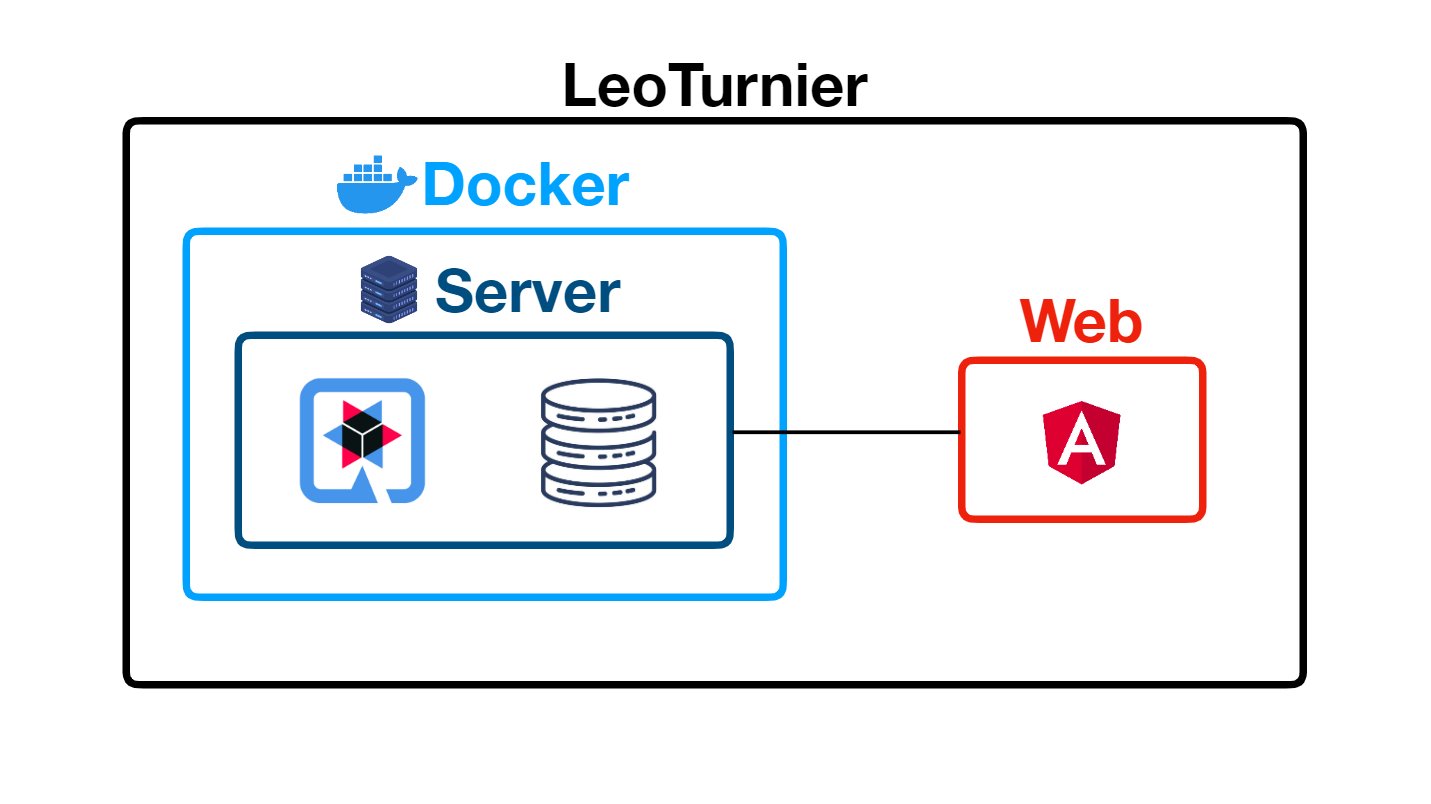
\includegraphics[scale=0.25]{pics/system_architecture.png}
\end{figure}


\section{Verwendete Technologien}

\subsection{Git}

\includegraphics[scale=0.05]{pics/git.png}

Git ist das mit Abstand am weitesten verbreitete Versionskontrollsystem der Welt. Der Name Git wird aus der britischen 
Umgangssprache übersetzt und bedeutet "Blödmann.
\cite{sysarch-git-1}
Es ist ein Open-Source Projekt, 
das ursprünglich 2005 von dem Entwickler des Linux Betriebsystem-Kernels entwickelt wurde. Es ist außerdem mit sowohl mit 
Windows als auch Linux Systemen kompatibel und auch in vielen verschiedenen IDEs integriert. Git ist ein verteiltes Versionskontrollsystem, 
was bedeutet, dass der Versionsverlauf nicht nur an einem Ort gespeichert ist, wie es bei älteren Versionskontrollsystemen der Fall war, 
sondern in jeder Arbeitskopie der gesamte Verlauf aller Änderungen im Repository (Aufbewahrungsort) enthalten sind. 

\cite{sysarch-git-2}

\subsubsection{Was ist ein Versionskontrollsystem?}

Ein Versionskontrollsystem wie Git wird in der Softwareentwicklung verwendet, 
um Änderungen des Quellcodes zu speichern und zu verwalten. 
Hier gibt es drei Arten von Versionskontrollsystemen:
\cite{sysarch-git-2}
\begin{itemize}
 \item lokale Versionsverwaltung (Local Version Control System - LVCS): 
\end{itemize}
Hier werden Dateien lokal einfach nur in ein separates Verzeichnis kopiert.
\cite{sysarch-git-2}
\begin{itemize}
 \item zentrale Versionsverwaltung (Centralized Version Control System - CVCS):
\end{itemize}
Hier gibt es einen einen zentralen Server, der alle versionierten Dateien verwaltet und es Personen ermöglicht, 
Dateien von diesem zentralen Repository abzuholen und auf ihren PC zu übertragen.
\cite{sysarch-git-2}
\begin{itemize}
 \item verteilten Versionsverwaltung (Distributed Version Control System - DVCS):
\end{itemize}
Wie weiter oben schon angesprochen ist diese Variante jene, die von Git benutzt wird. Hier gibt es zwar ein zentrales Repository, 
aber jede Person  hat eine Kopie des Repositories und somit die vollständigen Projektdaten.
\cite{sysarch-git-2}

\subsubsection{Git Befehle}

Git verwendet zum verwalten eines Repositories das Terminal, hierzu gibt es einige wichtige Befehle. Zuerst kann man mit "git init" ein leeres Repository erstellen 
oder ein existierendes nochmal initialisieren, alternativ kann man mit "git clone" ein existierendes Repository kopieren. Damit ein File von Git gespeichert werden
kann, muss man es zunächst mit "git add" zum Repository hinzufügen, das ganze kann dann mit "git rm" wieder rückgängig gemacht werden. Mit "git status" wird der 
momentane Status aller Files im Repository angezeigt, dass heißt, ob das File neu im Repository ist, ob es seit dem letzten Mal Speichern verändert wurde, oder ob es 
erst garnicht im Repository vorhanden ist. Nun kann man mit "git commit" den momentanen Status des Repositories als neue Version speichern und mit "git push" an ein "remote" 
Repository senden. Als letzter wichtiger Befehl gilt noch "git branch", hiermit kann man das Repository in verschiedene "Branches" aufteilen und so 
neue Features getrennt voneinander entwickeln, und diese dann mit "git merge" im Hauptbranch zusammenfügen.
\cite{sysarch-git-2}

\subsection{Github}

\includegraphics[scale=0.05]{pics/github.png}

Github ist ein Cloud-basiertes Repository Hosting Service, das die verteilte Versionskontrolle von Git zur verfügung stellt. Es wurde 2008 von Chris Wanstrath, P. J. Hyett, 
Scott Chacon und Tom Preston-Werner gestartet. Zu dem Zeitpunkt war Git noch relativ unbekannt, wesshalb es noch keine anderen Optionen gab. Die Software wurde in der 
Programmiersprache "Ruby on Rails and Erlang" entwickelt. 
\cite{sysarch-github-1}
Das Ziel von Github ist es, eine benutzerfreundliche Oberfläche für Git zur verfügung zu stellen, mit der man auch mit weniger technischem Wissen die Vorteile von Git ausnutzen kann.
\cite{sysarch-github-2}
Als Unternehmen verdient GitHub Geld, indem es gehostete private Code-Repositories sowie andere geschäftsorientierte Pläne verkauft, 
die es Unternehmen erleichtern, Teammitglieder und Sicherheit zu verwalten.
\cite{sysarch-github-2}

\subsubsection{Github Issues}

Github verfügt über einen integrierten issue tracken, mit dem sich Issues auf GitHub verwalten lassen. Ein Issue ist eine 
Aufgabe im Projekt, die mit dem Titel kurz, und dann in der Beschreibung genauer beschrieben wird, und einem bestimmten Entwickler 
zugeteilt wird. Ein Issue kann den Status "open" oder "closed" haben, "open" bedeutet, dass die Aufgabe noch nicht erfüllt wurde, und 
"closed" bedeutet dass die Aufgabe schon erfüllt ist. Github Issues haben gegenüber von anderen issue trackern vorallem einem Vorteil, 
weil es direkt dort ist, wo auch der Quellcode zu finden ist, jedoch ist es weit nicht so mächtig wie manch andere Optionen, wesshalb 
sich bei dieser Arbeit nicht für Github Issues entschieden wurde.
\cite{sysarch-github-3}

\subsubsection{Github Actions}

GitHub Actions ist ein in Github integriertes Tool, um Prozesse in einem Softwareprojekt zu automatisieren. 
Dadurch kann man Workflows für dein Repository erstellen. Ein Workflow besteht aus einem oder mehreren Jobs, 
wobei ein Job aus einem oder mehreren Schritten besteht. Man kann festlegen, ob Workflows in einem Container oder in einer virtuellen 
Maschine ausgeführt werden sollen. Die Ausführung kann unter den gängigen Betriebssystemen Windows, Linux und macOS erfolgen. 
Workflows werden durch Events wie beispielsweise ein Push auf das Repository ausgelöst und ausgeführt. Wenn ein Workflow ausgeführt wird, 
arbeitet er alle seine Jobs, sowie Schritte ab und erstellt dir ein umfangreiches Feedback mit Logs und Ausführungszeiten. 
Das Feedback kann individuell für jeden Schritt angepasst werden. Eine Action wird in der Web-Oberfläche von GitHub erstellt. 
Praktischerweise kann eine erstellte Action geteilt und wiederverwendet werden.
\cite{sysarch-github-4}

\subsubsection{Github Packages}

Ein Package ist ein wiederverwendbares Stück Software, das von einer globalen Registry in die lokale Umgebung eines Entwicklers heruntergeladen und 
in den Anwendungscode integriert werden kann. Da Pakete als wiederverwendbare "Bausteine" fungieren und in der Regel allgemeine Anforderungen erfüllen 
(z. B. API-Fehlerbehandlung), können sie zur Verkürzung der Entwicklungszeit beitragen. Github Packages ist ein Package Managing Service, 
der die Veröffentlichung von Packages erleichtert und vollständig in GitHub integriert ist. Alles befindet sich an einem Ort, 
sodass man zum Suchen und Veröffentlichen von Paketen dieselben Such-, Browsing- und Verwaltungstools verwenden kann wie für Repositories.
\cite{sysarch-github-5}

\subsection{Intellij IDEA}

\includegraphics[scale=0.05]{pics/intellijIdeaLogo.png}

IntelliJ IDEA ist eine intelligente, kontextsensitive IDE für Java und andere JVM-Sprachen wie Kotlin, Scala und Groovy, die sich für zahlreiche 
Anwendungsbereiche eignet. Auch bei der Entwicklung von Full-Stack-Webanwendungen hilft IntelliJ IDEA Ultimate mit leistungsstarken integrierten Tools, 
Unterstützung für JavaScript und verwandte Technologien sowie erweiterte Unterstützung für gängige Frameworks wie Spring, Spring Boot, Jakarta EE, Micronaut, 
Quarkus oder Helidon. Darüber hinaus kann IntelliJ IDEA mit kostenlosen Plugins von JetBrains erweitern, um die IDE mit anderen Programmiersprachen wie 
Go, Python, SQL, Ruby und PHP einzusetzen.

\subsection{WebStorm}
\includegraphics[scale=0.025]{pics/WebStormLogo.svg.png}


Obwohl es möglich wäre mit Intellij ein Angular Projekt zu entwickeln haben wir uns bei der Frontend Entwicklung 
für die IDE Webstorm entschieden. Diese ist genauso wie Intellij von Jetbrains doch enthält mehr support für die 
Programmiersprachen JavaScript und TypeScript, sowie einen Built-in Debugger für Client-Side JavaScript und Node.js 

\subsection{Quarkus}

\includegraphics[scale=0.015]{pics/quarkusLogo.png}

Quarkus ist ein Framework zur Erstellung von Java-Anwendungen mit dem Java speziell für Container optimiert wird. 
Es bietet eine effektive Plattform für Serverless-, Cloud- und Kubernetes Umgebungen. Der Hersteller Redhat wirbt 
auch mit schnellen Startzeiten und geringen Speicherplatzverbrauch. Dise erzielt Quarkus dadurch dass es den Code schon Buildvorgangs verabeitet.

\subsection{Maven}
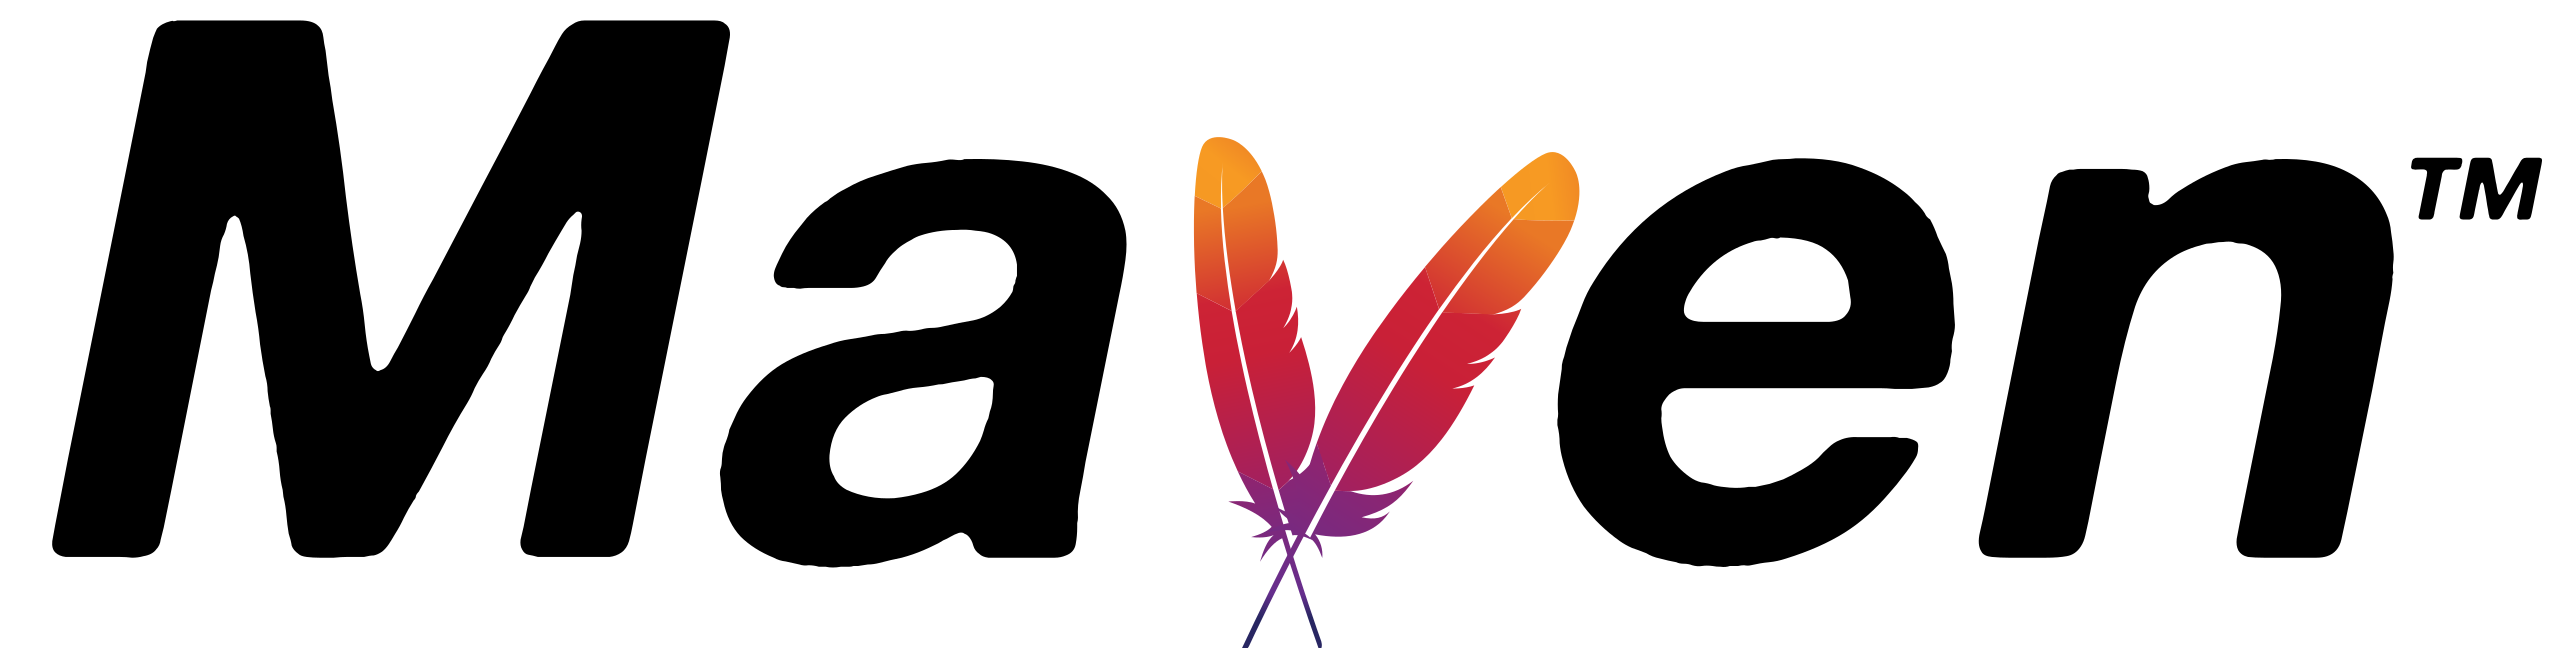
\includegraphics[scale=0.015]{pics/apacheMavenLogo.svg.png}

Maven ist ein Build Atomation Tool welches hauptsächlich für Java verwendet wird und folgt dem Ansatz Konvention vor Konfiguration. TODO


\subsection{Angular}

\includegraphics[scale=0.02]{pics/angularLogo.svg.png}

Angular ist ein Client-Side JavaScript Framework zur Erstellung von Single-Page-Webapplications. 
Seine komponentenbasierte Architektur welche View und Logik trennt macht es für den Entwickler leicht 
Applikationen zu warten und testen. Dabei verwendet Angular TypeScript für den Code-Behind und HTML als Auszeichnungssprache. 
Die vielen gut integrierten Libraries decken Features wie Routing, Verwaltung von Formulare und Client-Server Kommunikation ab. 

\subsection{PostgreSQL}

\includegraphics[scale=0.015]{pics/postgresqlLogo.svg.png}

PostgreSQL ist eine objektrelationale Datenbank welche sich durch ihre Stabilität und freie Verfügbarkeit auszeichnet. 
Sie hält sich dabei sehr eng an den SQL-Standard. Es werden eine Vielzahl von Datentypen und Operatorn unterstützt und 
Entwickler können auch eigene Datentypen definieren. Ein weitetere großer Vorteil von PostgreSQL ist auch dass es auf 
jeder Hardware und auf beinahe jedem Betriebsystem läuft. 
\subsection{Docker}

\includegraphics[scale=0.05]{pics/dockerLogo.png}

Docker ist eine Software zur Containervirtualisierung . Die Container sind voneinander isoliert und haben ihre eigene Software, 
Libraries sowie Konfigurationsdatein. Kommunizieren können sie über vorher genau definierte Kanäle. Da alle Container 
auf dem selben OS-Kernel laufen brauchen sie weniger Resourcen wie eine Virtuele Maschine.

\begin{spacing}{1}
\chapter{Technologien}\label{chapter:tech}
\end{spacing}
\section{Git}
\setauthor{Hain Lukas}

Git ist das mit Abstand am weitesten verbreitete Versionskontrollsystem der Welt. Der Name Git wird aus der britischen 
Umgangssprache übersetzt und bedeutet "Blödmann.
\cite{sysarch-git-1}

Es ist ein Open-Source Projekt, 
das ursprünglich 2005 von dem Entwickler des Linux Betriebsystem-Kernels entwickelt wurde. Es ist außerdem mit sowohl mit 
Windows als auch Linux Systemen kompatibel und auch in vielen verschiedenen IDEs integriert. Git ist ein verteiltes Versionskontrollsystem, 
was bedeutet, dass der Versionsverlauf nicht nur an einem Ort gespeichert ist, wie es bei älteren Versionskontrollsystemen der Fall war, 
sondern in jeder Arbeitskopie der gesamte Verlauf aller Änderungen im Repository (Aufbewahrungsort) enthalten sind. 
\cite{sysarch-git-2}

\subsection{Was ist ein Versionskontrollsystem?}

Ein Versionskontrollsystem wie Git wird in der Softwareentwicklung verwendet, 
um Änderungen des Quellcodes zu speichern und zu verwalten. 
Hier gibt es drei Arten von Versionskontrollsystemen:
\cite{sysarch-git-2}

\subsubsection{lokale Versionsverwaltung (Local Version Control System - LVCS)}
Hier werden Dateien lokal einfach nur in ein separates Verzeichnis kopiert.
\cite{sysarch-git-2}

\subsubsection{zentrale Versionsverwaltung (Centralized Version Control System - CVCS)}
Hier gibt es einen einen zentralen Server, der alle versionierten Dateien verwaltet und es Personen ermöglicht, 
Dateien von diesem zentralen Repository abzuholen und auf ihren PC zu übertragen.
\cite{sysarch-git-2}

\subsubsection{verteilten Versionsverwaltung (Distributed Version Control System - DVCS)}
Wie weiter oben schon angesprochen ist diese Variante jene, die von Git benutzt wird. Hier gibt es zwar ein zentrales Repository, 
aber jede Person  hat eine Kopie des Repositories und somit die vollständigen Projektdaten.
\cite{sysarch-git-2}

\subsection{Git Befehle}

Git verwendet zum verwalten eines Repositories das Terminal, hierzu gibt es einige wichtige Befehle. Zuerst kann man mit "git init" ein leeres Repository erstellen 
oder ein existierendes nochmal initialisieren, alternativ kann man mit "git clone" ein existierendes Repository kopieren. Damit ein File von Git gespeichert werden
kann, muss man es zunächst mit "git add" zum Repository hinzufügen, das ganze kann dann mit "git rm" wieder rückgängig gemacht werden. Mit "git status" wird der 
momentane Status aller Files im Repository angezeigt, dass heißt, ob das File neu im Repository ist, ob es seit dem letzten Mal Speichern verändert wurde, oder ob es 
erst garnicht im Repository vorhanden ist. Nun kann man mit "git commit" den momentanen Status des Repositories als neue Version speichern und mit "git push" an ein "remote" 
Repository senden. Als letzter wichtiger Befehl gilt noch "git branch", hiermit kann man das Repository in verschiedene "Branches" aufteilen und so 
neue Features getrennt voneinander entwickeln, und diese dann mit "git merge" im Hauptbranch zusammenfügen.
\cite{sysarch-git-2}

\subsection{Leistung}

Bei reiner Betrachtung der Leistungsmerkmale von Git, fällt auf, wie stark diese im Vergleich zu vielen Alternativen sind. Für die Commits neuer 
Änderungen, Branching, Merging und den Vergleich älterer Versionen wurde auf optimale Performance geachtet. Die in Git implementierten Algorithmen schöpfen 
aus umfassenden Kenntnissen häufiger Attribute echter Quellcode-Dateibäume, deren Modifizierung im Laufe der Zeit und den entsprechenden Zugriffsmustern.
\cite{sysarch-git-1}

\subsection{Sicherheit}

Bei der Konzipierung von Git gehörte die Integrität des verwalteten Quellcodes zu den obersten Prioritäten. Der Inhalt der Dateien sowie die wahren Beziehungen 
zwischen den Dateien und Verzeichnissen, Versionen, Tags und Commits – alle diese Objekte im Git-Repository werden mit einem kryptografisch sicheren Hashing-Algorithmus namens SHA1 gesichert. 
Auf diese Weise sind der Code und der Änderungsverlauf gegen versehentliche als auch vorsätzliche Änderungen geschützt und die vollständige Verfolgbarkeit des Verlaufs wird sichergestellt.
\cite{sysarch-git-1}

\subsection{Flexibilität}

Eines der wichtigsten Designziele von Git ist die Flexibilität. Git ist in mehrerer Hinsicht flexibel: in seinem Support verschiedener nicht-linearer Entwicklungs-Workflows, 
in seiner Effizienz sowohl bei kleinen als auch großen Projekten und in seiner Kompatibilität mit vielen bestehenden Systemen und Protokollen.
\cite{sysarch-git-1}

\subsection{Warum Git?}

Git verfügt über die Funktionen, Performance, Sicherheit und Flexibilität, die den Anforderungen der meisten Teams und einzelnen Entwicklern entsprechen. 
Auf diese Attribute von Git wurde oben schon eingegangen. In direkter Gegenüberstellung mit den meisten anderen Alternativen schneidet Git sehr gut ab.
\cite{sysarch-git-1}

\section{Github}
\setauthor{Hain Lukas}

Github ist ein Cloud-basiertes Repository Hosting Service, das die verteilte Versionskontrolle von Git zur verfügung stellt. Es wurde 2008 von Chris Wanstrath, P. J. Hyett, 
Scott Chacon und Tom Preston-Werner gestartet. Zu dem Zeitpunkt war Git noch relativ unbekannt, wesshalb es noch keine anderen Optionen gab. Die Software wurde in der 
Programmiersprache "Ruby on Rails and Erlang" entwickelt. 
\cite{sysarch-github-1}

Das Ziel von Github ist es, eine benutzerfreundliche Oberfläche für Git zur verfügung zu stellen, mit der man auch mit weniger technischem Wissen die Vorteile von Git ausnutzen kann.
Als Unternehmen verdient GitHub Geld, indem es gehostete private Code-Repositories sowie andere geschäftsorientierte Pläne verkauft, 
die es Unternehmen erleichtern, Teammitglieder und Sicherheit zu verwalten.
\cite{sysarch-github-2}

\subsection{Github Issues}

Github verfügt über einen integrierten issue tracken, mit dem sich Issues auf GitHub verwalten lassen. Ein Issue ist eine 
Aufgabe im Projekt, die mit dem Titel kurz, und dann in der Beschreibung genauer beschrieben wird, und einem bestimmten Entwickler 
zugeteilt wird. Ein Issue kann den Status "open" oder "closed" haben, "open" bedeutet, dass die Aufgabe noch nicht erfüllt wurde, und 
"closed" bedeutet dass die Aufgabe schon erfüllt ist. Github Issues haben gegenüber von anderen issue trackern vorallem einem Vorteil, 
weil es direkt dort ist, wo auch der Quellcode zu finden ist, jedoch ist es weit nicht so mächtig wie manch andere Optionen, wesshalb 
sich bei dieser Arbeit nicht für Github Issues entschieden wurde.
\cite{sysarch-github-3}

\subsection{Github Actions}

GitHub Actions ist ein in Github integriertes Tool, um Prozesse in einem Softwareprojekt zu automatisieren. 
Dadurch kann man Workflows für dein Repository erstellen. Ein Workflow besteht aus einem oder mehreren Jobs, 
wobei ein Job aus einem oder mehreren Schritten besteht. Man kann festlegen, ob Workflows in einem Container oder in einer virtuellen 
Maschine ausgeführt werden sollen. Die Ausführung kann unter den gängigen Betriebssystemen Windows, Linux und macOS erfolgen. 
Workflows werden durch Events wie beispielsweise ein Push auf das Repository ausgelöst und ausgeführt. Wenn ein Workflow ausgeführt wird, 
arbeitet er alle seine Jobs, sowie Schritte ab und erstellt dir ein umfangreiches Feedback mit Logs und Ausführungszeiten. 
Das Feedback kann individuell für jeden Schritt angepasst werden. Eine Action wird in der Web-Oberfläche von GitHub erstellt. 
Praktischerweise kann eine erstellte Action geteilt und wiederverwendet werden.
\cite{sysarch-github-4}

\subsection{Github Packages}

Ein Package ist ein wiederverwendbares Stück Software, das von einer globalen Registry in die lokale Umgebung eines Entwicklers heruntergeladen und 
in den Anwendungscode integriert werden kann. Da Pakete als wiederverwendbare "Bausteine" fungieren und in der Regel allgemeine Anforderungen erfüllen 
(z. B. API-Fehlerbehandlung), können sie zur Verkürzung der Entwicklungszeit beitragen. Github Packages ist ein Package Managing Service, 
der die Veröffentlichung von Packages erleichtert und vollständig in GitHub integriert ist. Alles befindet sich an einem Ort, 
sodass man zum Suchen und Veröffentlichen von Paketen dieselben Such-, Browsing- und Verwaltungstools verwenden kann wie für Repositories.
\cite{sysarch-github-5}

\section{Intellij IDEA}
\setauthor{Hain Lukas}

IntelliJ IDEA ist eine intelligente, kontextsensitive IDE für Java und andere JVM-Sprachen wie Kotlin, Scala und Groovy, die sich für zahlreiche 
Anwendungsbereiche eignet. Auch bei der Entwicklung von Full-Stack-Webanwendungen hilft IntelliJ IDEA Ultimate mit integrierten Tools, 
Unterstützung für JavaScript und verwandte Technologien sowie erweiterte Unterstützung für gängige Frameworks wie Spring, Spring Boot, Jakarta EE, Micronaut, 
Quarkus oder Helidon. Darüber hinaus kann IntelliJ IDEA mit Plugins von JetBrains erweitern, um die IDE mit anderen Programmiersprachen wie 
Go, Python, SQL, Ruby und PHP einzusetzen. 
\cite{sysarch-intellij-1}

\subsection{Was ist eine IDE?}

Eine IDE (Integrated Development Environment) oder integrierte Entwicklungsumgebung ist Software für die Anwendungsentwicklung, 
die gängige Entwicklertools in einer zentralen grafischen Oberfläche vereint. Eine typische IDE besteht aus folgenden Komponenten:
\cite{sysarch-intellij-2}

\subsubsection{Quellcode-Editor }
Ein Texteditor, der eine Programmierung von Software-Code mit folgenden Features unterstützt: 
Syntaxhervorhebung mit visuellen Hinweisen, sprachspezifische Autovervollständigung und eine Bug-Prüfung, während der Code geschrieben wird.
\cite{sysarch-intellij-2}

\subsubsection{Automatisierung lokaler Builds}
Dienstprogramme, mit denen sich einfache wiederholbare Aufgaben im Rahmen der Entwicklung lokaler Software-Builds zur Nutzung durch 
die Entwickler automatisieren lassen, wie beispielsweise die Kompilierung von Quell- in Binärcode, dessen Paketierung und die Ausführung automatischer Tests.
\cite{sysarch-intellij-2}

\subsubsection{Debugger}
Ein Programm zur Prüfung anderer Programme, mit dem sich die Position von Bugs im Originalcode grafisch anzeigen lässt.
\cite{sysarch-intellij-2}


\subsection{Codeanalyse}

Intellij bietet intelligente Programmierhilfen an. Durch eine Indizierung des Quellcodes legt die IDE eine virtuelle 
Karte des Projekts an. Anhand der Informationen in dieser virtuellen Karte kann sie Fehler erkennen, kontextabhängige Completion-Vorschläge anbieten oder
Refactorings durchführen.
\cite{sysarch-intellij-1}


\subsection{Versionsverwaltung}

IntelliJ IDEA unterstützt die gängigen Versionsverwaltungen (VCS) wie Git, Subversion, Mercurial und Perforce. 
Man kann ein VCS-Projekt direkt auf dem Startbildschirm klonen, die Unterschiede zwischen zwei Revisionen untersuchen, Branches verwalten, 
Commits durchführen und pushen, Konflikte bereinigen oder den Verlauf überprüfen. 
\cite{sysarch-intellij-1}


\subsection{JVM-Frameworks}

IntelliJ IDEA Ultimate bietet Unterstützung für Frameworks und Technologien zur Entwicklung von Anwendungen und Microservices. 
Die IDE bietet spezielle Unterstützung unter anderem für Quarkus, Spring, Spring Boot, Jakarta EE, JPA und Reactor.
\cite{sysarch-intellij-1}


\section{WebStorm}
\setauthor{Ecker Benjamin}


Obwohl es möglich wäre mit Intellij ein Angular Projekt zu entwickeln haben wir uns bei der Frontend Entwicklung 
für die IDE Webstorm entschieden. Diese ist genauso wie Intellij von Jetbrains doch enthält mehr support für die 
Programmiersprachen JavaScript und TypeScript, sowie einen Built-in Debugger für Client-Side JavaScript und Node.js 

TODO


\section{Java}
\setauthor{Hain Lukas}

Java ist nicht nur eine Programmiersprache, sondern ebenso ein Laufzeitsystem, was Oracle durch den Begriff Java Platform verdeutlichen will. 
So gibt es neben der Programmiersprache Java durchaus andere Sprachen, die eine Java-Laufzeitumgebung ausführen, etwa diverse Skriptsprachen wie 
Groovy, JRuby, Jython, Kotlin oder Scala. Skriptsprachen auf der Java-Plattform werden immer populärer; sie etablieren eine andere Syntax, nutzen aber die JVM und die Bibliotheken.
Zu der Programmiersprache und JVM kommt ein Satz von Standardbibliotheken für Datenstrukturen, Zeichenkettenverarbeitung, Datum/Zeit-Verarbeitung, grafische Oberflächen, 
Ein-/Ausgabe, Netzwerkoperationen und mehr. Das bildet die Basis für höherwertige Dienste wie Datenbankanbindungen oder Webservices. Integraler Bestandteil der Standardbibliothek 
seit Java 1.0 sind weiterhin Threads. Sie sind leicht zu erzeugende Ausführungsstränge, die unabhängig voneinander arbeiten können. 
Mittlerweile unterstützen alle populären Betriebssysteme diese »leichtgewichtigen Prozesse« von Haus aus, sodass die JVM diese parallelen Programmteile nicht nachbilden muss, 
sondern auf das Betriebssystem verweisen kann. Auf den neuen Multi-Core-Prozessoren sorgt das Betriebssystem für eine optimale Ausnutzung der Rechenleistung, da Threads wirklich nebenläufig arbeiten können.
\cite{sysarch-java-1}

\subsection{Java Life Cycle}

Der Life Cycle (Lebenszyklus) eines Java Programms gibt an, was genau mit dem Programm passiert, wie es vom Quellcode, den man in der IDE eingibt, zum Maschinenode wird, der aus 0 und 1 besteht.
Es gibt 3 Hauptphasen im Lebenszyklus:
\begin{itemize}
    \item Bearbeitung des Programms
    \item Kompilierung des Quellcodes
    \item Ausführung des Byte Codes
\end{itemize}
Zuerst wird der Code in die IDE bzw. den Editor eingegeben, wenn man damit fertig ist, wird der Code in einem oder mehreren Files gespeichert. Diese Files haben die Endung ".java". 
Als nächstes wird das Programm kompiliert. Der Name des Java Compilers ist "javac". Der Input an den Compiler ist der Java Quellcode aus den ".java" Files, der Output des Compilers 
ist Platform-unabhängiger Code namens "Byte Code". Das File, das vom Compiler generiert wurde, hat die Endung ".class". Als letztes wird das Programm ausgeführt. Der Bytecode, der vom Compiler 
generiert wurde, wird von der "Java Virtual Mashine" oder JVM ausgeführt, der input an die JVM ist der Bytecode aus dem ".class" File, der Output ist Maschinenode, bestehend aus 0 und 1, und wird von der CPU ausgeführt.
\cite{sysarch-java-2}
\begin{figure}[H]
    \centering
    \caption{Java Life Cycle}
    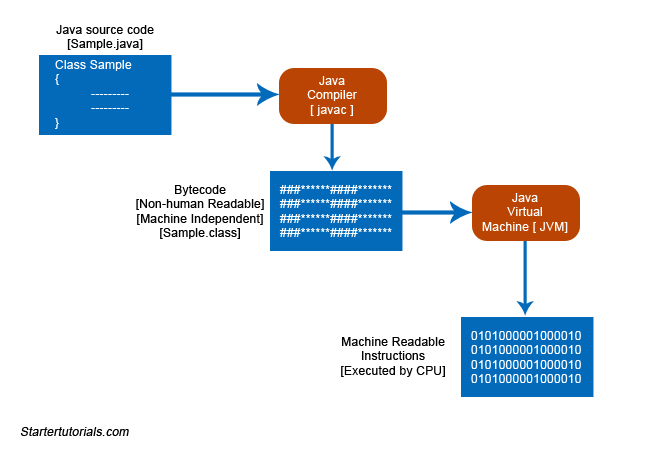
\includegraphics[scale=0.6]{pics/java-life-cycle.jpg}
\end{figure}

\section{TypeScript}
\setauthor{Ecker Benjamin}

TODO

\section{Quarkus}
\setauthor{Hain Lukas}

Quarkus ist ein Kubernetes-natives Full-Stack Java Framework für JVMs (Java Virtual Machines) und native Kompilierung, mit dem Java speziell für Container optimiert wird. 
Es bietet eine effektive Plattform für Serverless-, Cloud- und Kubernetes-Umgebungen. Quarkus wurde speziell für beliebte Java-Standards, Frameworks und Libraries wie Eclipse MicroProfile und Spring
sowie für Apache Kafka, RESTEasy (JAX-RS), Hibernate ORM (JPA), Spring, Infinispan, Camel und viele mehr konzipiert.
Die Dependency-Injection-Lösung von Quarkus basiert auf CDI (Contexts and Dependency Injection) und bietet ein Framework, mit dessen Hilfe die Funktionalität 
erweitert und ein Framework konfiguriert, gebootet und in Ihre Anwendung integriert werden kann. 

Quarkus wurde als benutzerfreundliches Tool konzipiert und integriert Funktionen, die keine oder nur wenig Konfiguration erfordern.
Entwickler können die passenden Java Frameworks für ihre Anwendungen auswählen, die dann im JVM-Modus laufen oder kompiliert und im nativen Modus ausgeführt werden können.
Das ganz auf Entwickler abgestimmte Quarkus integriert außerdem folgende Funktionen:
\begin{itemize}
    \item Live-Codierung zur umgehenden Prüfung der Auswirkungen von Code-Änderungen sowie eine schnelle Problembehebung
    \item Einheitliche imperative und reaktive Programmierung mit einem eingebetteten gemanagten Event Bus
    \item Einheitliche Konfiguration
    \item Einfaches Generieren nativer Programmdateien
\end{itemize}
Ob man die Anwendungen auf einer Public Cloud oder in einem intern gehosteten Kubernetes-Cluster hosten, Eigenschaften wie ein schneller 
Start sowie ein niedriger Speicherverbrauch sind wichtig, um die Gesamtkosten für das Hosting niedrig zu halten.
Quarkus wurde auf Basis einer Container-first-Philosophie entwickelt und soll so einen niedrigen Speicherverbrauch und schnelle Startzeiten auf folgende Weise ermöglichen:
\begin{itemize}
    \item Erstklassiger Support für Graal/SubstrateVM
    \item Metadaten-Verarbeitung gleichzeitig mit dem Build
    \item Reduzierung der Reflektionsnutzung
    \item Preboot nativer Images
\end{itemize}
Bei der Anwendungsentwicklung mit Quarkus wird im Vergleich zum traditionellen Java nur ein Zehntel des Speichers belegt. Dazu bietet es bis zu 300 Mal 
schnellere Startzeiten. Beide Aspekte ermöglichen eine deutliche Reduzierung der Kosten für Cloud-Ressourcen.
Quarkus ist so konzipiert, dass bei der Anwendungsentwicklung der bewährte imperative Code problemlos mit dem nicht-blockierenden reaktiven Code kombiniert werden kann.
Dies erweist sich als nützlich sowohl für Java-Entwickler, die an das imperative Modell gewöhnt sind und auch dabei bleiben möchten, und all diejenigen, die einen cloudnativen/reaktiven Ansatz bevorzugen.
Das Quarkus-Entwicklungsmodell lässt sich flexibel an alle zu erstellenden Anwendungstypen anpassen.
Quarkus ist eine effiziente Lösung zur Ausführung von Java in dieser neuen Welt von Serverless-Architekturen, Microservices, Containern, Kubernetes, 
Function-as-a-Service (FaaS) und Clouds, weil es für all diese Technologien entwickelt wurde.
\cite{sysarch-quarkus-1}

\subsection{RESTEasy}

RESTEasy ist ein JBoss/Red Hat-Projekt, das verschiedene Frameworks zur Verfügung stellt, die bei der Erstellung von RESTful Web Services und RESTful Java-Anwendungen unterstützen. 
Es ist eine Implementierung der Jakarta RESTful Web Services, einer Spezifikation der Eclipse Foundation, die eine Java-API für RESTful Web Services über das HTTP-Protokoll bereitstellt.
Darüber hinaus implementiert RESTEasy auch die MicroProfile REST Client Spezifikation API.

RESTEasy kann in jedem Servlet-Container ausgeführt werden, aber eine engere Integration mit WildFly Application Server und Quarkus 
ist ebenfalls verfügbar, um die Benutzerfreundlichkeit in diesen Umgebungen zu verbessern.
\cite{sysarch-quarkus-2}

\subsection{Hibernate ORM with Panache}

Bei Hibernate handelt es sich um ein Framework zur Abbildung von Objekten auf relationalen Datenbanken für die Programmiersprache Java - es wird auch als Object Relational Mapping Tool bezeichnet. 
Hibernate ist in der Programmiersprache Java implementiert und steht als Open Source zur freien Verfügung. Hibernate nutzt das Konzept der Reflexion, um so zur Laufzeit einer Software sogenannte 
Meta- Informationen über die Struktur von Objekten und die zugrunde liegenden Klassen zu ermitteln, die dann auf die Tabellen einer Datenbank abgebildet werden.
\cite{sysarch-quarkus-3}

\section{Apache Maven}
\setauthor{Hain Lukas}

Maven ist ein Build-Tool der Apache Software Foundation für die Projektverwaltung. Entwickler können damit Java-Projekte automatisieren. Maven ist ein Teil der Apache Software Foundation und wird von dieser gehostet. 
Das Tool ist aus einem Teil des Jakarta-Projekts hervorgegangen. Maven vereinfacht den Softwareerstellungsprozess, bietet ein einheitliches System für die Entwicklerarbeit, hochwertige Projektinformationen, 
Richtlinien für das Festlegen von Best Practices und erleichtert die Migration zu neuen Funktionen durch mehr Transparenz. Maven beschreibt sowohl, wie Software gebaut wird, als auch deren Abhängigkeiten. 
Apache hilft sowohl bei der Verwaltung von Projekten und dient als Tool zum Verständnis. Es hilft also dabei, den Zustand eines Projekts sehr schnell darzustellen.
Das Programm wird von Entwicklern und Projektmanagern von Java-Anwendungsprojekten verwendet. Das Tool kann nützlich sein, um den aktuellen Zustand eines Projektes 
auf einem Blick für technisch weniger versierte Personen, wie Führungspersönlichkeiten und Investoren, zusammenzufassen. Maven basiert auf dem Objektmodell. 
Projekte werden als eine Pom.xml-Datei gespeichert. 

Das Tool verwaltet Projekt-Builds, Reporting und Dokumentation aus der zentralen XML-Informationsbasis. 
Mit seiner Standard-Plug-in-Architektur kann Maven über Standard-Input mit so gut wie jeder Anwendung zusammenarbeiten.
Maven vereinfacht den Prozess für das Erstellen von Java-Anwendungen erheblich, da Nutzer den Status des Projektes viel einfacher einschätzen können.
Der Name Maven kommt aus dem Jiddischen und bedeutet Akkumulator von Wissen. Obwohl Maven das Entwickeln von Software anhand von Konventionen ermöglicht, 
sind reproduzierbare Builds derzeit kein Feature. Die Entwickler arbeiten aber daran. 
\cite{sysarch-maven-1}

\section{Angular}
\setauthor{Ecker Benjamin}

Angular ist ein Client-Side JavaScript Framework zur Erstellung von Single-Page-Webapplications. 
Seine komponentenbasierte Architektur welche View und Logik trennt macht es für den Entwickler leicht 
Applikationen zu warten und testen. Dabei verwendet Angular TypeScript für den Code-Behind und HTML als Auszeichnungssprache. 
Die vielen gut integrierten Libraries decken Features wie Routing, Verwaltung von Formulare und Client-Server Kommunikation ab. 

TODO

\section{Nginx}
\setauthor{Ecker Benjamin}

TODO

\section{PostgreSQL}
\setauthor{Hain Lukas}

Dieses DBMS (Datenbank-Managementsystem) bietet eine liberale Lizenz, flexiblen Umgang mit Datentypen, ist skalierbar und vielseitig nutzbar.
Der Definition nach ist PostgreSQL ein „objektrelationales“ Datenbank-Managementsystem (DBMS). Es ist Open Source und orientiert sich sehr eng am SQL-Standard. Bestehende SQL-Anwendungen 
können durch den ANSI-SQL-Standards ohne großen Aufwand integriert werden. Die Funktionsweise entspricht dem klassischen Client-Server-Prinzip, bei dem unterschiedliche Clients Anfragen an den Datenbankserver senden.
In der Praxis ist es mit PostgreSQL möglich, komplexere Anwendungen und Workloads zu entwickeln und zu betreiben als mit anderen Lösungen. 
Es unterstützt eine Vielzahl Datentypen und Operatoren. Entwickler können hier bei Bedarf eigene Datentypen definieren. PostgreSQL ist nicht nur für Webanwendungen sehr gut geeignet, es kann auch große Enterprise-Datenbanken abbilden. 
PostgreSQL findet auch in Desktop-Systemen Einsatz: Es ist das Datenbanksystem von Linux und macOS. Diese Systeme liefern das Datenbanksystem standardmäßig mit.
\cite{sysarch-postgresql-1}

\subsection{Vorteile}

\subsubsection{Offene Lizenz}
Einer der größten Vorteile von PostgreSQL ist die offene Lizenz. Es ist unter der eigenen PostgreSQL-Lizenz veröffentlicht. Generell fallen dabei keine Lizenzkosten an. 
Diese liberale Lizenz erlaubt es, das System beliebig zu vertreiben. Änderungen müssen nicht der Community zur Verfügung gestellt werden. Die Verwendung von PostgreSQL hat 
keine nachgelagerten Auswirkungen darauf, wie Weiterentwicklungen und darauf basierende Lösungen verwendet werden dürfen oder veröffentlicht werden müssen.
\cite{sysarch-postgresql-1}

\subsubsection{Großes Potenzial}

Die Datenbankgröße ist nicht durch das System begrenzt, sondern einzig durch den zur Verfügung stehenden Speicher. Da Postgres flexibel und kompatibel aufgebaut ist, 
können eine Vielzahl an Anwendungen auf diese Datenbanklösung bauen. Dazu bietet PostgreSQL die Möglichkeit, 
Trigger einzusetzen und bietet Schnittstellen zu vielen verschiedenen Programmiersprachen, was den Einsatzzweck und die Zusammenarbeit mit unterschiedlichsten Anwendungen potenziell vielfältig macht.
\cite{sysarch-postgresql-1}

\subsubsection{Sichere Replikation}

Ein weiterer wichtiger Punkt ist die detaillierte Zugriffskontrolle und sichere Datenreplikation. In der Praxis ist je nach Anwendungsfall asynchrone oder synchrone Replikation möglich: 
Synchrone Replikation, um sicherzustellen, dass kritische Transaktionen auf beiden Servern ausgeführt wurden. Asynchrone Replikation für maximale Geschwindigkeit bei weniger kritischen Transaktionen. 
Ein weiterer Vorteil ist die freie Wahl der Hardware und des Server-OS. PostgreSQL kann auf diversen Linux-Distributionen, BSD, Windows oder macOS 
gehostet werden.
\cite{sysarch-postgresql-1}

\section{Docker}
\setauthor{Hain Lukas}

Die Docker-Technologie verwendet den Linux Kernel und seine Funktionen wie Cgroups und namespaces, um Prozesse zu isolieren, damit diese unabhängig voneinander ausgeführt werden können. 
Diese Unabhängigkeit ist der Zweck der Container – die Fähigkeit, mehrere Prozesse und Apps getrennt voneinander betreiben zu können. 
So wird die Infrastruktur besser genutzt und gleichzeitig die Sicherheit bewahrt, die sich aus der Arbeit mit getrennten Systemen ergibt.
Containertools, einschließlich Docker, arbeiten mit einem Image-basierten Bereitstellungsmodell. Das macht es einfacher, eine Anwendung oder ein Paket von Services mit all deren 
Abhängigkeiten in mehreren Umgebungen gemeinsam zu nutzen. Docker automatisiert außerdem die Bereitstellung der Anwendung 
(oder Kombinationen von Prozessen, die eine Anwendung darstellen) innerhalb dieser Container-Umgebung. Diese Tools bauen auf Linux-Containern auf 
und geben den Nutzern so nie dagewesenen Zugriff auf Anwendungen. Sie ermöglichen eine deutlich schnellere Bereitstellung und Kontrolle von Versionen sowie deren Verbreitung.
\cite{sysarch-docker-1}

\subsection{Vorteile}

\subsubsection{Modularität}

Der Docker-Ansatz für die Containerisierung konzentriert sich darauf, nur einen Teil der Anwendung für eine Reparatur oder Aktualisierung außer Betrieb zu nehmen, 
ohne dass die gesamte Anwendung außer Betrieb genommen werden muss. Zusätzlich zu diesem auf Microservices basierenden Ansatz können Sie Prozesse 
in mehreren Apps gemeinsam verwenden – so ähnlich wie bei einer serviceorientierten Architektur (SOA).
\cite{sysarch-docker-1}

\subsubsection{Layer und Image-Versionskontrolle}

Jedes Docker-Image besteht aus einer Reihe von Layern. Diese Layer werden in einem einzelnen Image vereint. Wenn sich das Image ändert, wird ein Layer erstellt. 
Jedes Mal, wenn ein Nutzer einen Befehl wie run oder copy eingibt, wird ein neuer Layer erstellt. Mit Docker werden diese Layer für neuer Container wiederverwendet, 
was die Entwicklung enorm beschleunigt. Zwischenzeitliche Änderungen werden von den Images gemeinsam verwendet, was die Geschwindigkeit, Größe und Effizienz weiter verbessert. 
Versionskontrolle ist ein fester Bestandteil des Layering. Bei jeder neuen hat man im Prinzip ein eingebautes Änderungsprotokoll und damit volle Kontrolle über die Container-Images.
\cite{sysarch-docker-1}

\subsubsection{Rollback}

Das Beste am Layering ist wahrscheinlich das Rollback, also das Zurücksetzen auf die vorherige Version. Jedes Image hat Layers. Wenn man mit der aktuellen Iteration eines Image nicht zufrieden ist, kann man einfach
auf die vorherige Version zurücksetzen. Dieser Ansatz unterstützt eine agile Entwicklung und sorgt, was die Tools angeht, 
für eine kontinuierliche Integration und Bereitstellung (Continuous Integration/Continuous Deployment - CI/CD).
\cite{sysarch-docker-1}

\subsubsection{Schnelle Bereitstellung}

Neue Hardware bereitzustellen und zum Laufen zu bringen, dauerte normalerweise Tage und war mit einem enormen Aufwand verbunden. Mit Docker-basierten Containern kann die Bereitstellung auf Sekunden reduziert werden. 
Indem man für jeden Prozess einen Container erstellt, kann man ähnliche Prozesse schnell mit neuen Apps teilen. Und da zum Hinzufügen oder Verschieben eines Containers das 
Betriebssystem nicht gebootet werden muss, sind die Bereitstellungszeiten wesentlich kürzer. Darüber hinaus kann man bei dieser Entwicklungsgeschwindigkeit 
einfach und kosteneffizient Daten erstellen und die von den Containern erzeugten Daten ohne Bedenken löschen.
Die Docker-Technologie ist also ein granularer, kontrollierbarer, auf Microservices basierter Ansatz, der deutlich effizienter ist.
\cite{sysarch-docker-1}

\subsection{Einschränkungen}

Docker für sich allein ist für die Verwaltung einzelner Container bestens geeignet. Wenn man beginnt, mehr und mehr Container und containerisierte Apps zu verwenden, 
die in Hunderte von Bestandteilen zerlegt sind, können die Verwaltung und Orchestrierung sehr schwierig werden. Irgendwann muss man einen Schritt zurückgehen und Container gruppieren, 
um Dienste wie Vernetzung, Sicherheit, Telemetrie usw. in den Containern bereitzustellen.
\cite{sysarch-docker-1}

\section{KeyCloak}
\setauthor{Hain Lukas}

Keycloak ist eine Open-Source-Lösung für Identity und Access Management (IAM), die auf die Entwicklung moderner Anwendungen und Services ausgerichtet ist.
\cite{sysarch-keycloak-1}

\subsection{Single Sign-on und Single Sign-out}

Möchte man mehrere Applikationen oder Dienste verwenden, so sind in der Regel bei jeder Applikation separate Logins erforderlich. Beim Single Sign-on (SSO) geht es jedoch darum, 
dass nur eine einzige Authentifizierung notwendig ist (beim ersten Zugriff auf eine der Applikationen). Dies geschieht dadurch, dass die Applikation die Benutzerin bzw. 
den Benutzer auf eine zentrale Keycloak-Instanz weiterleitet, welche die Login-Maske für die angesprochene Applikation ausgibt und in der Folge die Authentifizierung durchführt.
Nach erfolgreicher Anmeldung wird zur Applikation weitergeleitet. Werden anschließend andere Software-Systeme im SSO-Verbund verwendet, dann weiß Keycloak, dass die Benutzerin bzw. 
der Benutzer bereits authentifiziert ist und fordert keine weitere Anmeldung mehr. Zusätzlich verfügt Keycloak auch über eine Kerberos-Bridge, sodass die Anmeldung am Arbeitsrechner 
für die Authentifizierung ausreicht. Darüber hinaus unterstützt Keycloak auch ein Single Sign-out: Nach der Abmeldung erfolgt das automatische Ausloggen aus allen Applikationen im SSO-Verbund.
\cite{sysarch-keycloak-2}

\subsection{Unterstützung von Standardprotokollen}

Keycloak unterstützt Standardprotokolle wie OAuth 2.0 (nur Autorisierung) und das darauf basierende OpenID Connect (Autorisierung und Authentifizierung). 
Daneben wird mit SAML 2.0 ein weiteres Standardprotokoll unterstützt, welches ähnliche Anforderungen wie OpenID Connect (OIDC) abdeckt. 
Im Gegensatz zu OIDC existiert SAML jedoch schon länger, basiert auf XML und setzt zum Erreichen von Integrität und Vertraulichkeit digitale Signaturen und entsprechende Zertifikate ein.
\cite{sysarch-keycloak-2}

\subsection{Account Management Console}

Ein Self-Service-Portal ermöglicht es Benutzern, ihre Daten jederzeit selbst zu verwalten. Keycloak bietet ein solches Portal unter dem Namen „Account Management Console“ an. 
So können z. B. Passwortänderungen selbständig durchgeführt werden, ohne von Administratoren abhängig zu sein.
\cite{sysarch-keycloak-2}

\subsection{Admin Console}

Die Admin Console umfasst im Wesentlichen die Konfiguration von:
\begin{itemize}
    \item Realms (jeweils abgegrenzte Bereiche, für die die anderen in dieser Aufzählung genannten Aspekte einzeln konfiguriert bzw. verwaltet werden können)
    \item Clients (Applikationen und Dienste)
    \item Benutzerdatenquellen (siehe User Federation)
    \item weiteren Identity Providern (siehe Identity Brokering und Social Login)
    \item die Verwaltung von lokal in Keycloak angelegten Benutzern, Benutzern aus anderen Datenquellen, Benutzergruppen und Rollen
\end{itemize}
\cite{sysarch-keycloak-2}

\subsection{Client-Adapter}

Clients kommunizieren über die angebotenen Standardprotokolle mit Keycloak. Damit diese Kommunikation nicht für jeden Client – evtl. sogar redundant – selbst implementiert werden muss, 
gibt es für eine Vielzahl an Technologien und Frameworks fertige Client-Adapter, die sich einfach in die eigene Anwendung integrieren lassen und die Kommunikation mit Keycloak übernehmen. 
\cite{sysarch-keycloak-2}


\begin{spacing}{1}
\chapter{Umsetzung Frontend}\label{chapter:implementation_frontend}
\end{spacing}
\section{Home-Page - Rollen:Alle}
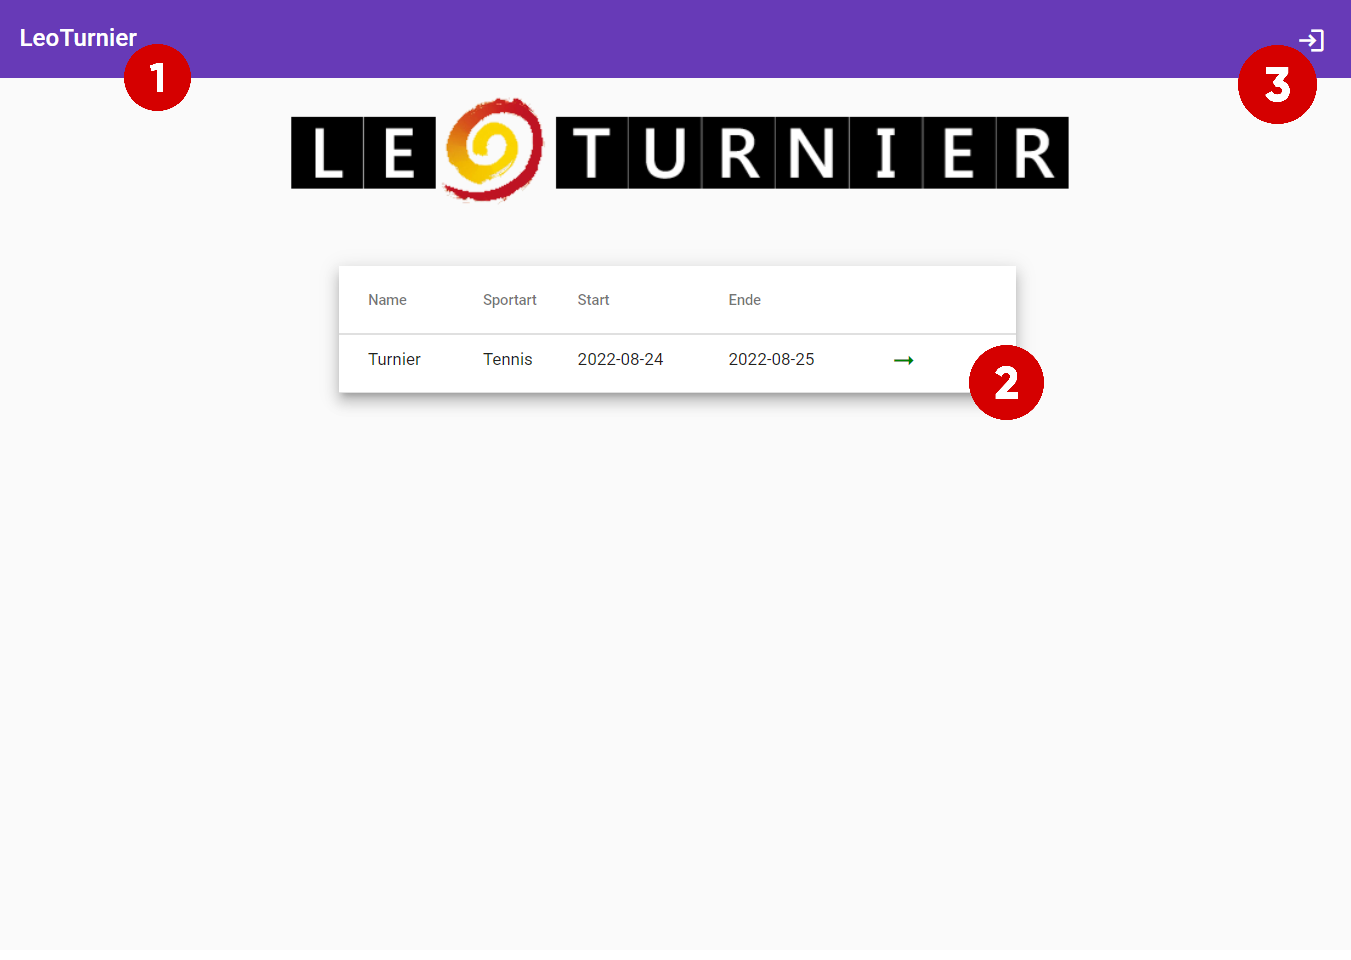
\includegraphics[scale=0.4]{pics/user-guide/homepage.png}
\bigskip


\includegraphics[scale=0.05]{pics/user-guide/numbers/number-1.png} \begin{LARGE} Titel \end{LARGE}

Links oben wird dauerhaft der Titel LeoTurnier gezeigt dieser dient auch gleichzeitig als Homebutton,
also kommt man per Knopfdruck immer wieder auf diese Seite.
\bigskip



\includegraphics[scale=0.05]{pics/user-guide/numbers/number-2.png} \begin{LARGE} Laufenden Turniere \end{LARGE}

In dieser Tabelle werden alle laufenden Turniere angezeigt. Zu jedem Turnier werden die Sportart, das Startdatum und das Enddatum angezeigt,
sollten diese eingetragen sein. (\textit{Nur der Name und der Modus sind zur Erstellung nötig})

Mit dem rechten grünen Pfeil kommen Sie zur Tournament-View-Page(5.2) des jeweiligen Turniers.
\bigskip

\newpage

\includegraphics[scale=0.05]{pics/user-guide/numbers/number-3.png} \begin{LARGE} Login Button \end{LARGE}

Um Turniere zu erstellen und verwalten zu können ist es nötig sich vorher einzuloggen. Mit diesem Button sollten Sie direkt zum Keycloak weitergeleitet werden um sich mit ihrem Username und Password zu authorisieren.
Danach werden Sie zur Login-Page(5.3) weitergeleitet werden.

\newpage
\section{Tournament-View-Page - Rollen: Alle}

Es gibt 2 Arten von Tournament-View-Pages:
\begin{itemize}
    \item Tree-View (für den Elimination Modus)
    \item Table-View (für den Round Robin Modus)
\end{itemize}

\subsection{Tree-View}
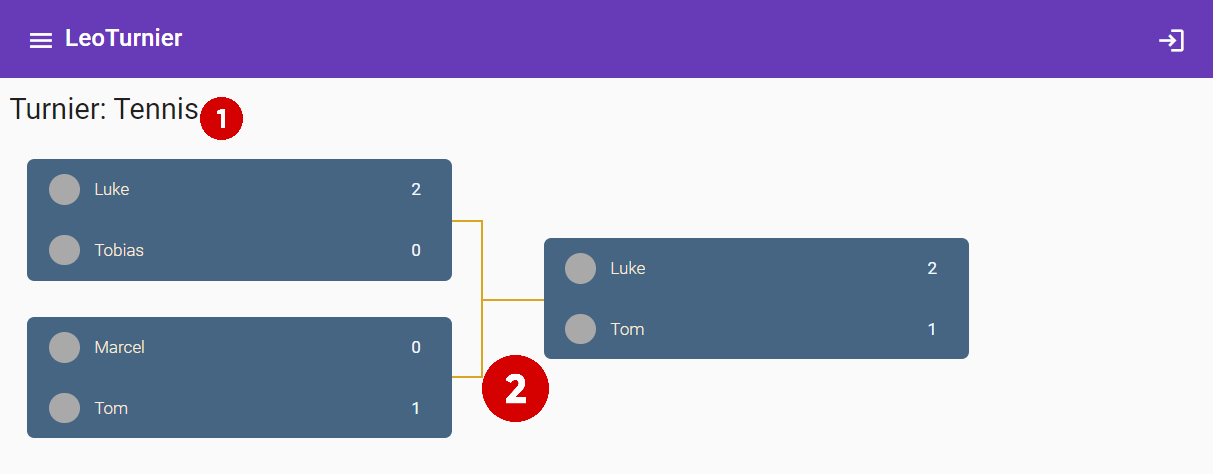
\includegraphics[scale=0.4]{pics/user-guide/tree-view.png}
\bigskip


\includegraphics[scale=0.05]{pics/user-guide/numbers/number-1.png} \begin{LARGE} Info \end{LARGE}

Hier finden Sie eine kurze Info zum Turniernamen und Sportart
\bigskip


\includegraphics[scale=0.05]{pics/user-guide/numbers/number-2.png} \begin{LARGE} Turnierbaum \end{LARGE}

Hier finden Sie den Turnierbaum, dieser zeigt alle Ergebnisse bzw. aktuellen Spielstände eines Turnieres an.
Im Screenshot sehen Sie eine der einfachsten Formen eines Turnierbaums mit 4 Spielern. Sollte der Turnierbaum bei
steigender Spieleranzahl zu groß werden um alles auf einen Bildschirm zu sehen verwenden Sie bitte den Slider am unterem Bildschirmrand.

Das Neuladen des Turniers funktioniert auf dieser Seite nicht. Um den aktuellsten Stand des Turniers zu bekommen navigieren Sie zurück auf die Home-Page und wieder auf den grünen Pfeil.
\section{Login-Page - Rollen: Admin,Tournament-Organizer}
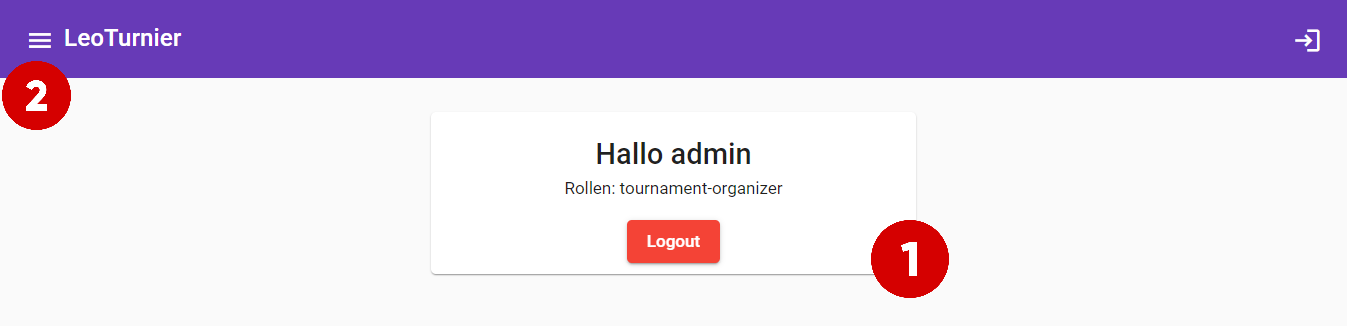
\includegraphics[scale=0.4]{pics/user-guide/login-page.PNG}
\bigskip


\includegraphics[scale=0.05]{pics/user-guide/numbers/number-1.png} \begin{LARGE} Rollen und Logout Button \end{LARGE}

Hier finden Sie alle Ihnen zugewiesenen Rollen sowie einen Logout-Button der ihre Session beendet und Sie zurück zur Home-Page leitet.
\bigskip


\includegraphics[scale=0.05]{pics/user-guide/numbers/number-2.png} \begin{LARGE} Navigation-Burger \end{LARGE}

Nachdem Sie jetzt eingeloggt sind erscheint oben rechts ein Nav-Burger. Per Knopfdruck zeigt dieser Ihnen nun eine Liste aller Pages die zur
Turnierverwaltung nötig sind.

\newpage
\section{Player-Page - Rollen:Admin,Tournament-Organizer}
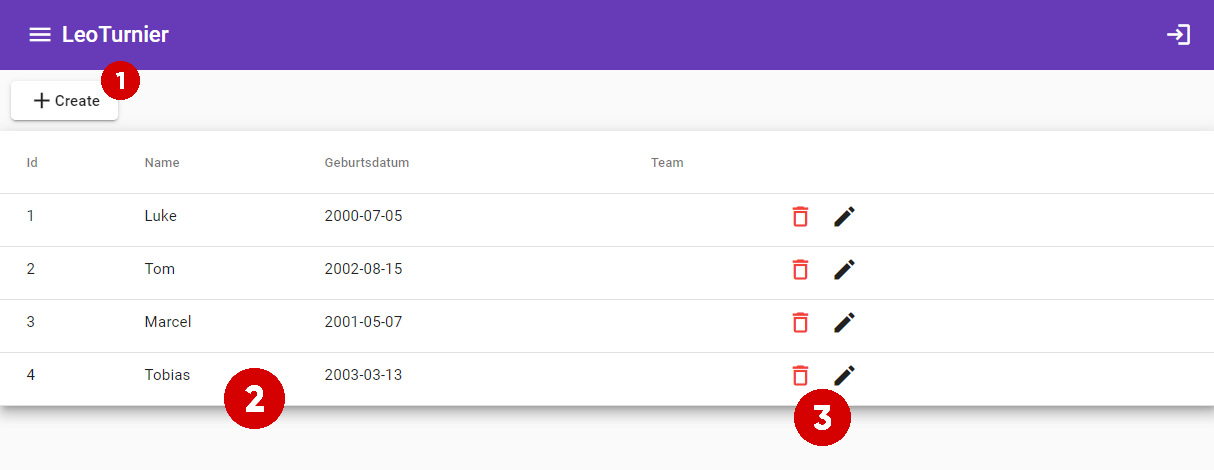
\includegraphics[scale=0.425]{pics/user-guide/player-overview-page.PNG}
\bigskip


\includegraphics[scale=0.05]{pics/user-guide/numbers/number-1.png} \begin{LARGE} Create-Button \end{LARGE}

Button zum Erstellen neuer Spieler und leitet Sie zur Player-Details-Page(5.4.1).

\bigskip

\includegraphics[scale=0.05]{pics/user-guide/numbers/number-2.png} \begin{LARGE} Players \end{LARGE}

In dieser Tabelle werden alle Spieler mit ihren Details angezeigt. Zu jedem Spieler werden hier seine Id, Name, Geburtsdatum und zugehöriges Team angezeigt,
sollten dieser vorhanden sein. (\textit{Nur der Name ist zur Erstellung nötig})

\bigskip

\includegraphics[scale=0.05]{pics/user-guide/numbers/number-3.png} \begin{LARGE} Actions \end{LARGE}

Diese Spalte beinhaltet zwei Icon-Buttons:
\begin{itemize}
    \item 
\includegraphics[scale=0.3]{pics/user-guide/delete-icon.PNG} Löschen eines Spieler (Sie müssen diese Aktion zwei mal bestätigen)
    \item
\includegraphics[scale=0.3]{pics/user-guide/edit-icon.PNG}Updaten eines Spieler(Sie werden danach zur Player-Details-Page(5.4.1)geleitet)
\end{itemize}
\subsection{Player-Details-Page}
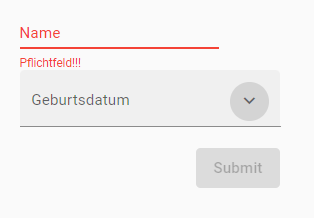
\includegraphics[scale=0.8]{pics/user-guide/player-create-page.PNG}

Diese Page ist zum Erstellen und Updaten von Spielern. Die Mindestanforderungen sind hierbei nur ein Name.


\section{Team-Page - Rollen:Admin,Tournament-Organizer}
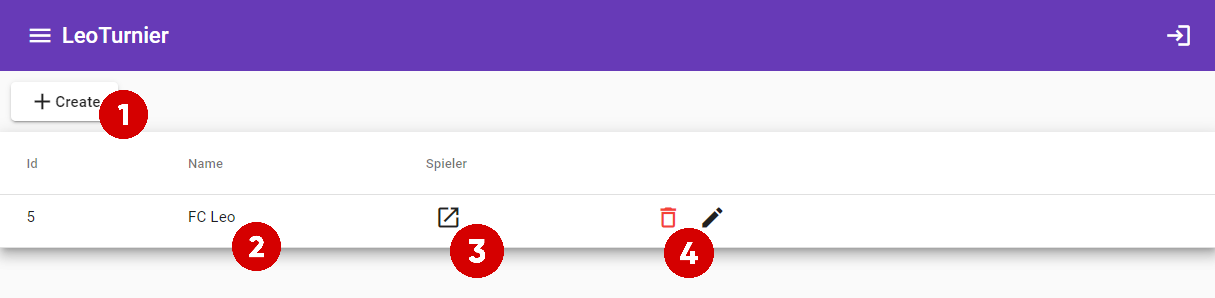
\includegraphics[scale=0.44]{pics/user-guide/team-overview-page.PNG}
\bigskip


\includegraphics[scale=0.05]{pics/user-guide/numbers/number-1.png} \begin{LARGE} Create-Button \end{LARGE}

Button zum Erstellen neuer Teams und leitet Sie zur Team-Details-Page(5.5.1).

\bigskip

\includegraphics[scale=0.05]{pics/user-guide/numbers/number-2.png} \begin{LARGE} Teams \end{LARGE}

In dieser Tabelle werden alle Teams mit ihren Details angezeigt. Zu jedem Team werden hier seine Id, Name und zugehörige Spieler angezeigt,
sollten dieser vorhanden sein. (\textit{Nur der Name ist zur Erstellung nötig})

\bigskip

\includegraphics[scale=0.05]{pics/user-guide/numbers/number-3.png} \begin{LARGE} Spieler \end{LARGE}

In der Spalte Spieler finden Sie einen Icon-Button zu einem PopUp-Fenster welches eine Liste aller Spieler des Teams anzeigt.

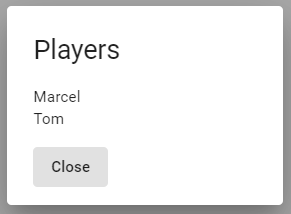
\includegraphics[scale=0.5]{pics/user-guide/teams-player-popup.PNG}

\bigskip

\includegraphics[scale=0.05]{pics/user-guide/numbers/number-4.png} \begin{LARGE} Actions \end{LARGE}

Diese Spalte beinhaltet zwei Icon-Buttons:
\begin{itemize}
    \item 
\includegraphics[scale=0.3]{pics/user-guide/delete-icon.PNG} Löschen eines Teams (Sie müssen diese Aktion zwei mal bestätigen)
    \item 
\includegraphics[scale=0.3]{pics/user-guide/edit-icon.PNG}Updaten eines Teams(Sie werden danach zur Team-Details-Page(5.5.1) geleitet)
\end{itemize}

\bigskip
\subsection{Team-Details-Page}
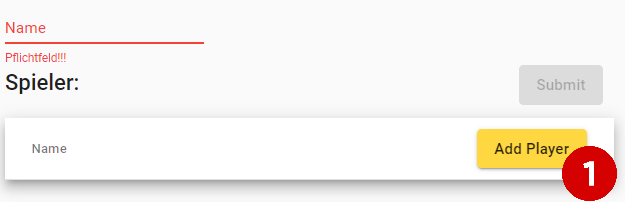
\includegraphics[scale=0.5]{pics/user-guide/team-create-page.PNG}

Diese Page ist zum Erstellen und Updaten von Spielern. Die Mindestanforderungen sind hierbei nur ein Name.

\bigskip

\includegraphics[scale=0.05]{pics/user-guide/numbers/number-1.png} \begin{LARGE} Add-Player \end{LARGE}

Bei Knopfdruck des Add-Player Button erscheint eine Liste aller Spieler die nicht in dem Team sind.
(\textit{Keine mehrfach Auswahl}) 

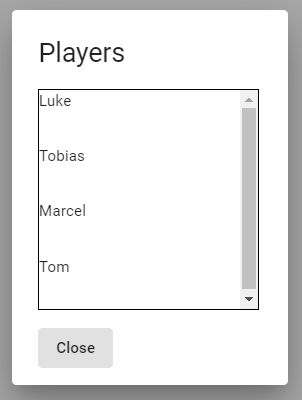
\includegraphics[scale=0.5]{pics/user-guide/add-player.PNG}

\newpage
\section{Tournament-Page Rollen:Admin,Tournament-Organizer}
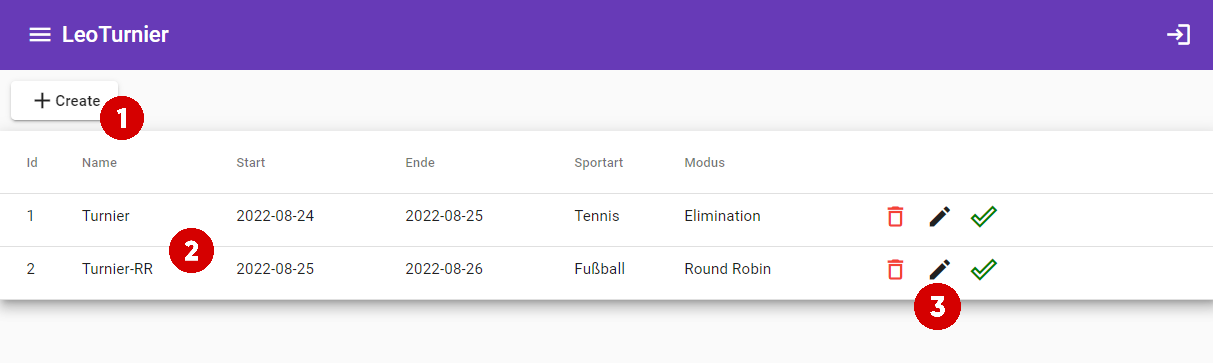
\includegraphics[scale=0.4]{pics/user-guide/tournament-overview-page.PNG}


\includegraphics[scale=0.05]{pics/user-guide/numbers/number-1.png} \begin{LARGE} Create-Button \end{LARGE}

Button zum Erstellen neuer Tournaments und leitet Sie zur Tournament-Details-Page(5.6.1).

\bigskip

\includegraphics[scale=0.05]{pics/user-guide/numbers/number-2.png} \begin{LARGE} Tournaments \end{LARGE}

In dieser Tabelle werden alle Tournaments mit ihren Details angezeigt. Zu jedem Tournament werden hier seine Id, Name, Startdatum, Enddatum, Sportart
und Turniermodus, sollten dieser vorhanden sein. (\textit{Nur der Name und der Modus sind zur Erstellung nötig})


\bigskip

\includegraphics[scale=0.05]{pics/user-guide/numbers/number-3.png} \begin{LARGE} Actions \end{LARGE}

Diese Spalte beinhaltet zwei bis drei Icon-Buttons:
\begin{itemize}
    \item 
\includegraphics[scale=0.3]{pics/user-guide/delete-icon.PNG} Löschen eines Tournaments (Sie müssen diese Aktion zwei mal bestätigen)
    \item 
\includegraphics[scale=0.3]{pics/user-guide/edit-icon.PNG}Updaten eines Tournaments (Sie werden danach zur Tournaments-Details-Page(5.6.1) geleitet)
    \item 
\includegraphics[scale=0.3]{pics/user-guide/submit-icon.PNG} Starten eines Tournaments (Sie müssen diese Aktion zwei mal bestätigen)
    \item 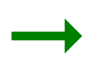
\includegraphics[scale=0.3]{pics/user-guide/go-to-icon.PNG} Leitet Sie zur Match-Overview-Page des Tournaments
\end{itemize}

\subsection{Tournament-Details-Page}
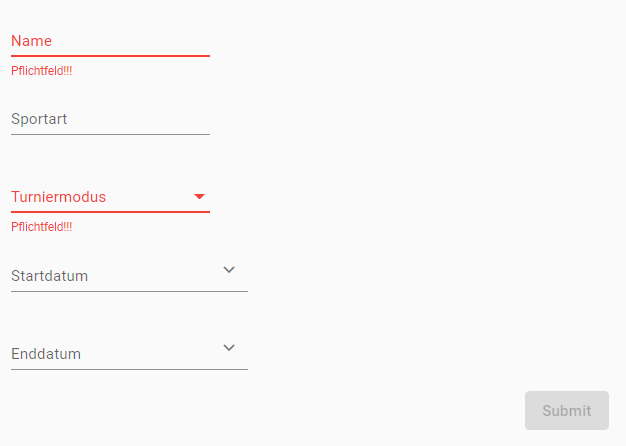
\includegraphics[scale=0.6]{pics/user-guide/tournament-create-page.PNG}

Diese Page ist zum Erstellen von Turnieren. Die Mindestanforderungen
sind hierbei nur ein Name und der Turniermodus.

Nachdem Sie ein Turnier erstellt haben erweitert sich die Tournament-Details-Page um die Funktion, Competitor(Spieler, Teams) für ein Turnier einzutragen.

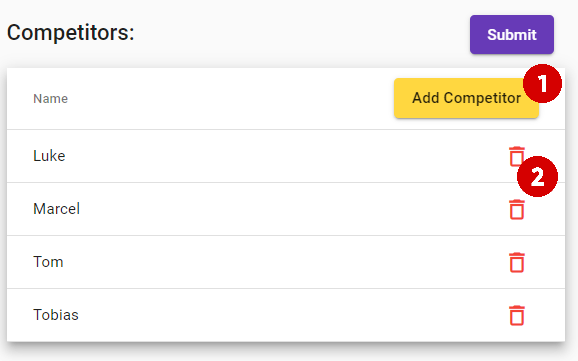
\includegraphics[scale=0.5]{pics/user-guide/tournament-add-player.PNG}

\includegraphics[scale=0.05]{pics/user-guide/numbers/number-1.png} \begin{LARGE} Add Competitor \end{LARGE}

Bei Knopfdruck des Add-Competitor Button erscheint eine Liste aller Spieler die nicht in dem Team sind.
(\textit{Keine mehrfach Auswahl})

\includegraphics[scale=0.4]{pics/user-guide/add-competitor.PNG}

\includegraphics[scale=0.05]{pics/user-guide/numbers/number-2.png} \begin{LARGE} Actions \end{LARGE}

Mit dem Icon-Button \includegraphics[scale=0.3]{pics/user-guide/delete-icon.PNG} löschen Sie die Teilnahme eines Competitors für das Turnier. (\textit{Nicht den Competitor})

\newpage
\section{Match-Overview-Page} 

\begin{spacing}{1}
\chapter{Umsetzung Backend}\label{chapter:implementation_backend}
\end{spacing}
\section{Datenmodell}
\setauthor{Hain Lukas}

\begin{figure}[H]
    \includegraphics[scale=1]{pics/backend/class_diagram.png}
    \caption{Class Diagram}
\end{figure}

Oben abgebildet ist das Datenmodell des Quarkus Backends. Anfangs erstellt man ein Turnier (Tournament), neben Namen, Startdatum und Enddatum 
wird hier noch der Turniermodus (TournamentMode) und die Sportart (SportType) festgelegt. Nun gibt man an, welche Teilnehmer/innen (Competitor) an diesem Turnier teilnehmen (Participation). 
Ein Competitor kann entweder ein einzelner Spieler (Player) oder ein Team von Spielern (Team) sein.
Wenn das Turnier gestartet wird, wird das Turnier in Phasen (Phase) unterteilt. In jeder Phase gibt es eine bestimmte Anzahl an Matches (Match), welche jeweils 2 Competitor haben und mithilfe von Nodes (Node) 
der jeweiligen Phase zugeordnet werden.

\section{Quarkus Backend}
\setauthor{Hain Lukas}

\subsection{Ordnerstruktur}

\begin{figure}[H]
    \includegraphics[scale=0.8]{pics/backend/quarkus_file_structure.png}
    \caption{Quarkus Ordnerstruktur}
\end{figure}

Nach dem erstellen eines Quarkus Projektes ist ein Großteil der Ordnerstruktur bereits im vorhinein gegeben. Das wichtigste File im Projekt befindet sich ganz im äußersten Ordner, nämlich das "pom.xml" File. 

\begin{figure}[H]
    \includegraphics[scale=0.6]{pics/backend/pom.xml.png}
    \caption{pom.xml}
\end{figure}

Hier werden nicht nur die Metadaten des Projekts angegeben, sondern auch die Dependencies, also alle externen Libraries, die die Applikation benötigt. 

Im "src" Ordner befinden sich ein "main" und ein "test" Ordner. Im "main" Ordner befindet sich der ganze Quellcode der Applikation, und im "test" Ordner befindet sich der Code, der den Quellcode auf seine richtigkeit prüft.
Im "main" Ordner befindet sich nun ein "docker" Ordner, auf den später noch eingegangen wird, ein "java" Ordner, in dem sich die Java Klassen der Applikation befindet, und ein "resources" Ordner, in dem weitere Files zu finden sind, 
auf die der Java Code eventuell zugreifen kann. Außerdem befindet sich im "resources" Ordner das "application.properties" File, in dem verschiedene Quarkus Konfigurationen zu finden sind.

\begin{figure}[H]
    \includegraphics[scale=0.6]{pics/backend/application.properties.png}
    \caption{application.properties}
\end{figure}

Die Konfigurationen sind aufgeteilt in Datasource (Datenbank), HTTP (Endpoints) und KeyCloak Konfigurationen. 

(Ist der Teil unten zu Basic?) (Der Teil unten gehört noch zur "Quarkus Ordnerstruktur" Abbildung, kann sein dass das etwas unklar ist, wie könnte ich das am besten machen?)

Die Java Klassen im "java" Ordner sind weiters in 5 verschiedene Ordner aufgeteilt. Im "entity" Ordner befinden sich alle Entitätsklassen der Applikation, also jene, die das Datenmodell (siehe Kapitel 6.1 Datenmodell) wiederspiegeln.
Die Klassen im "repository" sind die Schnittstelle zwischen der Quarkus Applikation und der Datenbank. Sie sind für die CRUD Operationen verantwortlich, also das Speichern, Auslesen, Verändern oder Löschen von Daten nach dem Schema der Entitätsklassen.
Außerdem befindet sich hier die Logik hinter den Turnieren. Die Klassen im "boundary" sind die Schnittstelle zum Frontend. Sie nehmen Requests, also Anforderungen, von außen an, 
führen die jeweilige Methode aus den Repository Klassen aus und liefern dann eine Response, also eine Antwort, zurück. Als nächstes gibt es die im "execution" Ordner, diese sind für die Durchführung der Turniere zuständig, hier befindet sich auch der Großteil der Logik. 
Zuletzt gibt es noch die Klassen in "dto" Ordner, diese sind Klassen, in denen Daten gespeichert werden können, die für die Logik in den Repository Klassen benötigt wird, jedoch nicht unbedingt Teil des Datenmodells sind.

\subsection{Entitätsklassen}

\begin{figure}[H]
    \includegraphics[scale=0.8]{pics/backend/entity_class.png}
    \caption{Entitätsklasse}
\end{figure}

Oben abgebildet ist eine der Entitätsklassen dieser Applikation, nämlich die Tournament Klasse. Ganz oben, über der Klasse, ist die Annotation "@Entity" zu finden, um sicherzustellen, dass die Klasse von JPA als Entitätsklasse erkannt wird, 
und das Library dafür eine Tabelle erstellt. Darunter befindet sich die "@Table" Annotation, die der Tabelle in der Datenbank ihren Namen gibt. Das Schema der Namensgebung von Tabellen lautet wie folgt: 
am Anfang steht immer die Abkürzung für den Tabellennamen, in diesem Fall ist das "T", danach kommt ein Unterstrich, gefolgt von dem Namen der Entitätsklasse in Großbuchstaben. 
In der Klasse selbst befinden sich nun die Klassenvariablen, welche von der Annotation "@Column" ihren Namen in der Datenbank verleiht. Das Schema der Namensgebung ist ähnlich, wie das der Tabellen: 
Anfangs die Abkürzung des Tabellennamens, dann ein Unterstrich als Trennung, gefolgt vom Namen der Klassenvariable, ebenfalls in Großbuchstaben. Die ID hat eine extra annotation, nämlich "@Id", 
das bedeutet dass sie der Primärschlüssel der Entitätsklasse ist. Wie der Wert der Id generiert wird, wird mit "@GeneratedValue" festgelegt. Außerdem steht bei den Variablen "tournamentmode" und "sportType" noch die "@ManyToOne" Annotation. 
Diese Felder werden dann in der Datenbank zu den Fremdschlüsseln auf andere Tabellen. Hier lautet das Namensschema wie folgt: Zuerst die Abkürzung der eigenen Klasse, 
dann der Name des Primärschlussels aus der Tabelle, auf die der Fremdschlüssel zeigt, wieder, getrennt durch einen Unterstrich.
Es gibt 4 Verschiedene Annotationen, die eine Beziehung zu anderen Tabellen herstellen:

\begin{itemize}
    \item @OneToOne
    \item @ManyToOne
    \item @OneToMany
    \item @ManyToMany
\end{itemize}

(wie könnte ich unten noch zu der "anderen" Klasse sagen?)

Die erste Mengenangabe steht immer für die eigene Klasse, die zweite steht für die andere Klasse. Diese braucht in diesem Fall natürlich auch die "@Entity" Annotation sowie einen Primärschlüssel. 
Bei "@OneToOne" und "@ManyToOne" wird in der Datenbank der Fremdschlüssel in der eigenen Tabelle erstellt, bei "@OneToMany" wird der Fremdschlüssel in der anderen Tabelle 
erstellt (hier muss die Variable, bei der die Annotation steht, auch eine Collection sein), und bei "@ManyToMany" wird eine Assotiationstabelle erstellt, in der sich dann 2 Fremdschlüssel befinden: 
einmal der au die Tabelle der eigenen Klasse, und einmal die der naderen Klasse.

Unter den Klassen befinden sich dann standardmäßig noch der Constructor sowie die Getter und Setter.

\subsection{Repositoryklassen}

\begin{figure}[H]
    \includegraphics[scale=0.8]{pics/backend/repository_class.png}
    \caption{Repositoryklasse}
\end{figure}

Wie oben schon erwähnt sind die Repositoryklassen die Schnittstelle zwischen Quarkus Backend und Datenbank, dies wird durch die "Hibernate ORM with Panache" Library ermöglicht. 
Außer ein paar Ausnahmen befinden sich hier nur die CRUD (Create - Read - Update - Delete) Operationen, als Create Operation fungiert hier die "add" Methode, 
als Read Operationen die "get" Methoden (getById, getByCompetitorId, getAll), als Update Operation die "modify" Methode und als Delete Operationen die "delete" und "clear". 
Über der Klasse befinden sich die Annotation "@ApplicationScoped" und "@Transactional". "@ApplicationScoped" ermöglicht es anderen Repositoryklassen, mithilfe von "@Inject" eine Instanz dieser Klasse zu injezieren, genau so, 
wie es diese Klasse weiter unten auch tut. Es wird zum Beispiel in der "add" Methode "TournamentRepository" Klasse (siehe Abbildung "add Methode aus TournamentRepository" unten) die 
der "SportTypeRepository" Klasse benötigt, da sich in der "Tournament" Klasse ein Fremdschlüssel auf die "SportType" Klasse befindet. Sollte also die Sportart, 
auf die dieser Fremdschlüssel zeigt, in der Datenbank nicht existieren, kommt es zu einer SQLException, wesshalb in der add Mehode von "TournamentRepository", 
bevor das Turnier selbst mit "persist" gespeichert wird, nocht die Sportart mithilfe der add Methode der "SportTypeRepository" Klasse in der Datenbank. 

\begin{figure}[H]
    \includegraphics[scale=0.8]{pics/backend/repository_add_function.png}
    \caption{add Methode aus TournamentRepository}
\end{figure}

Das gleiche passiert bei der "modify" Methode, wenn der Fremdschlüssel auf eine Sportart zeigt, die noch nicht existiert.

"@Transactional" wird verwendet, um in jeder Methode dieser Klasse vor den Ausführen eine neue Transaktion zu erstellen, und diese danach zu commiten. 
Wenn Daten in der Datenbank gespeichert, modifiziert oder gelöscht werden, werden diese Änderungen erst dann wirklich in die Datenbank übernommen, wenn eine Transaktion commitet wurde.

Das PanacheRepository ist eine Erweiterung aus dem "Hibernate ORM \textbf{with Panache}" Library, ohne Panache wäre theoretisch auch alles, was in den Repositoryklassen Implementiert wurde, möglich, jedoch etwas umständlicher.
Zum Beispiel gibt es ohne Panache die "persist" Methode nicht, in dem Fall müsste man eine "EntityManager" Instanz mithilfe von Dependency Injection injezieren, in davon dann die "persist" Methode hernehmen.
Auch andere Methoden, wie zum Beispiel "find" oder "listAll" wären ohne Panach nicht verfügbar, und müssten vom Entwickler selbst Implementiert werden.

\subsection{Serviceklassen}

\begin{figure}[H]
    \includegraphics[scale=0.6]{pics/backend/service_class.png}
    \caption{Serviceklasse}
\end{figure}

Die Serviceklassen sind die Schnittstelle zum Frontend, diesem stellen sie durch Endpoints, welche von Requests angesprochen werden, Daten aus der Datenbank zur Verfügung, dies wird durch die "RESTEasy" Library ermöglicht.
Über der Klasse wird mithilfe der Annotation "@Path" der URL Path zu den Endpoints dieser Klasse festgestellt. In der Klasse selbst wird zuerst eine Instanz des dazugehörigen Repositories injeziert. 
Danach folgt für jede CRUD Operation ein Endpoint. Es gibt verschiedene Arten von Endpoints, in dieser Applikation werden hauptsächlich 4 verwendet:

\begin{itemize}
    \item "@POST" bei Create Operationen
    \item "@PUT" bei Update Operationen
    \item "@GET" bei Read Operationen
    \item "@DELETE" bei Delete Operationen
\end{itemize}

"@RolesAllowed" gibt an, welche Rollen zugriff auf diesen Enpoint haben. Darauf wird im Kapitel KeyCloak noch genauer eingegangen. "@Consumes" und "@Produces" geben an, 
welche Art von Content in den Requests (@Consumes) bzw. den Responses (@Produces) übergeben werden soll. Außerdem wäre es noch möglich, den URL Path zu einem bestimmten Endpoint zu ändern, 
und zwar wieder mit der "@Path" Annotation. Bei den Parametern der Methoden gibt es manche mit der Annotation "@QueryParam", diese Annotation gibt an, dass dieser Parameter von der 
Request in der URL definiert wird. Zum Beispiel sieht die URL einer Request auf den GET Endpoint wie folgt aus:

\textbf{http://localhost:8080/api/tournament?id=1} 

Der Hostname ist in diesem Quarkus Backend "localhost", der Port 8080, der Root Path "api" wurde im "application.properties" File festgelegt, und der Path "tournament" wie erwähnt mit der "@Path" Annotation. 
Nach dem "?" werden immer die Queryparameter ("@QueryParam") übergeben, in diesem Fall die "id" mit dem Wert 1. Der Parameter "UriInfo" wird benötigt, um im Header der Response den Path zurückzugeben, 
mit dem man den neu hinzugefügten bzw. modifizierten Datensatz finden kann.

Was bei den Serviceklassen noch auffallend ist, ist dass es zum Beispiel für Read Operationen insgesammt nur einen Endpoint pro Serviceklasse gibt, obwohl es in den Repositoryklassen mehrere Get Methoden gibt (siehe Abbildung "Repositoryklasse").
Dies wird dadurch gelöst, dass Endpoints auch erfolgreich ausgeführt werden, wenn nicht alle Queryparameter in der URL definiert wurden, diese haben standardmäßig den Wert "null". Mit diesem Prinzib wird erreicht, dass mit dem gleichen URL Path 
verschiedene Read Operationen durchführen kann.

\begin{figure}[H]
    \includegraphics[scale=0.5]{pics/backend/service_get_function.png}
    \caption{get Methode aus TournamentService}
\end{figure}

Im obigen Beispiel hat man 3 Möglichkeiten:

\begin{itemize}
    \item keinen Query Parameter anzugeben, um alle Turniere auszulesen
    \item den "id" Query Parameter anzugeben, um nur das Turnier mit der angegebenen Id auszulesen
    \item den "competitorId" Query Parameter anzugeben, um alle Turniere auszulesen, in denen der Competitor mit der angegebenen Id dabei war.
\end{itemize}

Die einzige Entitätsklasse, für die es nur READ Endpoints gibt, ist die TournamentMode Klasse, Turniermodi werden beim Start des Backends mithilfe der "InitBean" Klasse 
automatisch in die Datenbank hinzugefügten, da diese für die Turnierdurchführung jeweils einzeln Implementiert werden müssen.

\subsection{Turnierdurchführung}

Für die Turnierdurchführung gibt es insgesammt 4 verschiedene Durchführungsklassen, eine für jeden Turniermodus (Elimination, Round Robin, Combination), und eine als Schnittstelle zu den Serviceklassen, welche aus den anderen 3 
die richtigen Methoden ausführen soll, abhängig davon, welchen Turniermodus das Turnier hat. 

\begin{figure}[H]
    \includegraphics[scale=0.65]{pics/backend/execution_startTournament.png}
    \caption{"startTournament" Methode der Execution Klasse}
\end{figure}

In der "startTournament" Methode zum Beispiel wird, nachdem alle vorherigen Matches usw. daraus gelöscht wurden, die "startTournament" Methode aus der dem TurnierModus entsprechenden Durchführungsklasse ausgeführt, 
bzw. im Falle des "Combination" Turniermodus die "startGroupPhase" Methode (mehr dazu weiter unten).

\subsection{Elimination}

Im Elimination Turniermodus scheidet nach einem Match der Verlierer sofort aus dem Turnier aus, und der Gewinner steigt in die nächste Runde auf. 
Das Ganze wiederholt sich so lange, bis nur noch ein/eine Teilnehmer/in übrig bleibt, dieser ist dann der Sieger des Turniers. So entsteht dann der klassische Turnierbaum.

\begin{figure}[H]
    \includegraphics[scale=0.5]{pics/backend/elimination/elimination_tree.png}
    \caption{Turnierbaum\cite{implementation-execution-1}}
\end{figure}

\subsubsection{Phases}

Ein Turnier ist in Phasen aufgeteilt, in der Abbildung oben ist jede Spalte von Matches eine Phase. Die Phasen eines Turniers werden mit der folgenden Methode eingefügt.

\begin{figure}[H]
    \includegraphics[scale=0.7]{pics/backend/elimination/elimination_insertPhases.png}
    \caption{Einfügen der Phasen im Elimination Modus}
\end{figure}

Zuerst wird die Anzahl der Phasen anhand der Teilnehmeranzahl berechnet. Dies erfolgt mit dem Logarithmus zur Basis 2 von der Teilnehmeranzahl (log\textsubscript{2}(n)). 
Da es in Java nicht möglich ist, die Basis eines Logarithmus frei zu wählen, wird stattdessen der Logarithmus der Teilnehmeranzahl dividiert durch den 
Logarithmus der Basis gerechnet, was zum gleichen Ergebnis kommt (log(n)/log(2)). Anschließend werden die Phasen numeriert in die Datenbank gespeichert, von 0 beginnend.

\subsubsection{Nodes}

Als nächstes werden zu jeder Phase Nodes eingefügt, diese bilden zusammen mit den Phasen das Grundgerüst des Turniers. 

\begin{figure}[H]
    \includegraphics[scale=0.48]{pics/backend/elimination/elimination_insertNodes.png}
    \caption{Einfügen der Nodes im Elimination Modus}
\end{figure}

Es wird rückwärts durch die Phasen des Turniers iteriert, sodass, die letzte Phase am Ende nur einen Node hat, nämlich das Finale.
Anschließend wird die Anzahl an Nodes für die momentane Phase berechnet, dies erfolgt mit der Rechnung 2 Hoch die Teilnehmeranzahl (2\textsuperscript{n}). 
Anschließend wird für jeden Node der "nextNode" gesetzt, das ist jener Node, in den der Sieger des Matches aus dem momentanen Nodes aufsteigen würde, 
und diese dann in die Datenbank eingefügt.

\subsubsection{Matches}

Zu jedem Node im Turnierbaum gehört ein Match, diese werden mit der folgenden Methode eingefügt.

\begin{figure}[H]
    \includegraphics[scale=0.48]{pics/backend/elimination/elimination_insertMatches.png}
    \caption{Einfügen der Matches im Elimination Modus}
\end{figure}

Diese Methode iteriert durch alle Nodes aus der ersten Phase durch, wobei durch "nodes.get(i / 2)" jede Node immer 2 Mal durchlaufen wird. 
Sollte eine Node noch kein Match haben, wird dieses hinzugefügt. Anschließend werden die Teilnehmer/innen, einer pro Durchlauf, also 2 pro Match, 
in die Matches eingefügt. 

\subsubsection{Seeding}

Um Turniere so spannend wie möglich zu gestalten, wird das sogenannte "Seeding" angewendet. Der Seed eines/einer Teilnehmers/in ist eine Einschätzung, wie gut dieser/diese Teilnehmer/in im vergleich zu den anderen im selben Turnier
ist. Somit ist der Seed 1 der/die beste Teilnehmer/in des Turniers, der Seed 2 der/die zweitbeste, usw. Mit Seeding will man erreichen, dass, angenommen der/die Teilnehmer/in mit dem niedrigeren Seed gewinnt immer gegen den/die 
mit dem höheren Seed, die Seeds 1 und 2, also die besten Teilnehmer/innen im Finale gegeneinander antreten. Würde man die Seeds einfach von oben nach unten in das Turnier einfügen, würde folgendes passieren.


\begin{figure}[H]
    \includegraphics[scale=0.33]{pics/backend/elimination/elimination_tree_seeded_wrong.png}
    \caption{Turnierbaum falsch geseedet\cite{implementation-execution-1}}
\end{figure}

Wie man sieht, treten die ersten beiden Seeds bereits im Halbfinale gegeneinander an, was für ein möglichst spannendes Turnier nicht wirklich wünschenswert ist. Aus diesem Grund werden die Teilnehmer/innen folgendermaßen zusammengeführt.

\begin{figure}[H]
    \includegraphics[scale=0.515]{pics/backend/elimination/elimination_tree_seeded.png}
    \caption{Turnierbaum richtig geseedet\cite{implementation-execution-1}}
\end{figure}

Der erste Seed tretet gegen den letzten an, der zweite gegen den vorletzten, usw. Auf diese weise ist es am wahrscheinlichsten, dass das finale Match so spannend wie möglich wird. 
Es steckt jedoch noch ein bisschen mehr dahinter. Sollte man es so machen, dass im ersten Match von oben der erste Seed gegen den letzten antritt, im zweiten von oben der zweite gegen den vorletzten, usw., 
würde bie größeren Turnieren spätestens in der zweiten Phase das selbe Problem nochmal auftreten.

\begin{figure}[H]
    \includegraphics[scale=0.25]{pics/backend/elimination/elimination_tree_seeded_wrong_big.png}
    \caption{großer Turnierbaum falsch geseedet\cite{implementation-execution-1}}
\end{figure}

Um dieses Problem zu beheben, wird beim Anordnen Rekursion verwendet.

\begin{figure}[H]
    \includegraphics[scale=0.5]{pics/backend/elimination/elimination_orderSeededCompetitors.png}
    \caption{Anordnen der Teilnehmer im Code}
\end{figure}

In der oberen Methode wird geprüft, ob die Anzahl der Teilnehmer/innen eine Hochzahl von 2 ist.
Außerdem wird angenommen, dass die Teilnehmer/innen nach Seed aufsteigend sortiert wurden. Nun wird die untere Methode ausgeführt, 
welche wie schon erwähnt Rekursion beinhaltet. Diese wird mit den folgenden Abbildungen erklärt.

\begin{figure}[H]
    \includegraphics[scale=0.8]{pics/backend/elimination/seeding_1.png}
    \caption{Anordnen der Teilnehmer 1}
    \includegraphics[scale=0.8]{pics/backend/elimination/seeding_2.png}
    \caption{Anordnen der Teilnehmer 2}
    \includegraphics[scale=0.8]{pics/backend/elimination/seeding_3.png}
    \caption{Anordnen der Teilnehmer 3}
\end{figure}

Im Grunde bewirkt dieser Code das gleiche, wie die Lösung von vorhin, nur mehrmals.
Angenommen das Turnier hat 8 Teilnehmer.
Der erste Durchlauf der Methode kümmert sich um die erste Phase, es werden die Seeds 1 und 8 zusammengeführt, 2 und 7, 3 und 6, und 4 und 5.
Der zweite Durchlauf kümmert sich nun um die zweite Phase. In der ersten Phase wird wie erwähnt davon ausgegangen, dass die Seeds 1 bis 4 in die zweite 
Phase aufsteigen, also sollten in der Phase die Seeds 1 und 4, und 2 und 3 zusammengeführt werden.
Dies wird erreicht, indem in der ersten Phase die Seeds 1 und 8 (also in der zweiten Phase nur Seed 1) mit den 
Seeds 4 und 5 (also in der zweiten Phase nur Seed 4) zusammengeführt werden. Das ganze wird so lange wiederholt, bis für jede zukünftige Phase richtig 
angeordnet wurde. Im Turnierbaum sieht es dass so aus.

\begin{figure}[H]
    \includegraphics[scale=0.25]{pics/backend/elimination/elimination_tree_seeded_big.png}
    \caption{großer Turnierbaum geseedet\cite{implementation-execution-1}}
\end{figure}

Im Backend gibt es 2 Möglichkeiten, Seeds and Teilnehmer/innen zu verteilen. Die erste Möglichkeit ist es, die Teilnehmer nach der durchnittlichen Plazierung aus vergangenen Turnieren zu sortieren, 
jedoch setzt das voraus, dass die Teilnehmer schon an Turniern teilgenommen haben. Sollte dies nicht der Fall sein, ist die zweite Möglichkeit, dass die Teilnehmer manuell vom Turnierorganisator sortiert werden.
Hier ist es allerdings von großer bedeutung, einen vertrauenswürdigen Turnierorganisator haben, denn, wie man oben sieht, je besser man im Vergleich zu anderen Teilnehmern eingeschätzt wird, desto leichtere Gegner wird man bekommen.

\subsubsection{Buy-Rounds}

Sollte die Anzahl der Teilnehmer/innen in einem Turnier keine Hochzahl von 2 sein, ist es nicht möglich, in der ersten Phase jedem/jeder Teilnehmer/in einen Gegner zu geben. 
Um dieses Problem zu lösen, steigen manche Teilnehmer automatisch in die zweite Phase auf, ohne ein Match gewonnen zu haben.

\begin{figure}[H]
    \includegraphics[scale=0.75]{pics/backend/elimination/elimination_buy_rounds.png}
    \caption{Turnierbaum mit Buy-Rounds\cite{implementation-execution-1}}
\end{figure}

Im Code wird das mit diesen Methoden erreicht.

\begin{figure}[H]
    \includegraphics[scale=0.65]{pics/backend/elimination/elimination_setBuyRounds.png}
    \caption{Buy-Rounds im Elimination Modus}
\end{figure}

Die untere Methode gibt alle Teilnehmer/innen des Turniers zurück, und zwar bereits nach Seed angeordnet. Besonders wichtig ist für Buy-Rounds der mittlere Teil der Methode. Angenommen ein Turnier hat 5 Teilnehmer/innen. 
Die nächste Hochzahl wäre in dem Fall 8, also befüllt diese Methode die Teilnehmerliste mit 3 "dummy" Teilnehmern, sodass die Teilnehmeranzahl eine Hochzahl von 2 ist. Dies ist notwendig, um die Teilnehmer/innen korrekt 
nach Seed anzuordnen. 

Nun sind jedoch 3 "dummy" Teilnehmer in der Teilnehmerliste, mit denen man nichts anfangen kann. Um diese kümmert sich nun die obere Methode. Jeder/jede Teilnehmer/in, der einen "dummy" Teilnehmer als Gegner hat, 
steigt automatisch in die zweite Phase auf, und spielt dort das erste Match.

\subsection{Round Robin}

Im Round Robin Turniermodus tritt jeder/jede Teilnehmer/in gegen jeden Teilnehmer an, egal, wie oft man gewinnt oder verliert. Somit entsteht hier kein Turnierbaum, sondern eher ein Turnierraster aus Matches.

\begin{figure}[H]
    \includegraphics[scale=0.5]{pics/backend/roundrobin/roundrobin_grid.png}
    \caption{Turnierraster\cite{implementation-execution-1}}
\end{figure}

\subsubsection{Phases}

Die Phasenanzahl im Round Robin Turniermodus ist etwas einfacher zu errechnen, als bei Elimination. Angenommen ein Turnier hat 4 Teilnehmer/innen, somit hat jeder/jede Teilnehmer/in insgesammt 3 Gegner. Da jeder/jede Teilnehmer/in in jeder Phase 
ein Match spielen kann, gibt es hier 3 Phasen, also die Teilnehmeranzahl - 1. Bei einer ungeraden Teilnehmeranzahl ist es jedoch etwas anders, da in jeder Phase ein/eine Teilnehmer keinen Gegner hat. Daher wäre hier die Phasenanzahl gleich 
der Teilnehmeranzahl.

\begin{figure}[H]
    \includegraphics[scale=0.5]{pics/backend/roundrobin/roundrobin_grid_uneven.png}
    \caption{Turnierraster mit ungerader Teilnehmeranzahl\cite{implementation-execution-1}}
\end{figure}

Die Rechnung im Code sieht folgendermaßen aus.

\begin{figure}[H]
    \includegraphics[scale=1]{pics/backend/roundrobin/roundrobin_insertPhases.png}
    \caption{Einfügen der Phasen im Round Robin Modus}
\end{figure}

\subsubsection{Nodes und Matches}

Da im Round Robin Turniermodus schon im Vorhinein bekannt ist, wer wann gegen wen antritt, werden hier Nodes und Matches gleichzeitig eingefügt. Dafür ist diese Methode verantwortlich.

\begin{figure}[H]
    \includegraphics[scale=0.6]{pics/backend/roundrobin/roundrobin_insertNodesAndMatches.png}
    \caption{Einfügen der Nodes und Matches im Round Robin Modus}
\end{figure}

Ein/eine Teilnehmer/in muss in jeder Phase gegen verschiedene Teilnehmer/innen antreten. In der ersten Phase nimmt die Methode aus der Teilnehmerliste den/die erste/n Teilnehmer/in, und den/die unmittelbar nächste, und fügt sie zusammen, 
so lange, bis keine Teilnehmer/innen mehr in der Liste sind. 

\begin{figure}[H]
    \includegraphics[scale=0.8]{pics/backend/roundrobin/matching_up_1.png}
    \caption{Round Robin Algorithmus 1}
\end{figure}

In der zweiten Phase wird wieder erste der/die Teilnehmer/in genommen, und diesmal der/die übernächste in der Liste. 

\begin{figure}[H]
    \includegraphics[scale=0.8]{pics/backend/roundrobin/matching_up_2.png}
    \caption{Round Robin Algorithmus 2}
\end{figure}

Dann wird der/die erste und der überübernächste, zusammengeführt.

\begin{figure}[H]
    \includegraphics[scale=0.8]{pics/backend/roundrobin/matching_up_3.png}
    \caption{Round Robin Algorithmus 3}
\end{figure}

Das ganze wird so lange wiederholt, bis jeder/jede Teilnehmer/in gegen jeden/jede andere Teilnehmer/in angetreten ist.

\subsubsection{Tie breakers}

Um zu vermeiden, dass am Ende eines Turniers 2 oder mehr Teilnehmer/innen gleich viele Matches gewonnen haben, und so auf dem gleichen Platz sind, 
wird bei den Plazierungen die Anzahl an Punkten ebenfalls in Betracht gezogen, jedoch besteht immernoch die Chance, dass sie ebenfalls die gleiche Anzahl an 
Punkten erziehlt haben. Sollte dies der Fall sein, ist es notwendig, sogenannte "Tie Breakers" auszuführen. Tie Breakers sind Matches, die nach den Hauptmatches 
des Turnier noch extra ins Turnier hinzugefügt werden, um den Punktegleichstand zwischen den Teilnehmer/innen zu beheben. Diese zählen für dei Plazierung nicht 
so viel wie ein normales Match, es kann also nicht sein, dass ein Teilnehmer 

\begin{spacing}{1}
\chapter{Zusammenfassung}
\end{spacing}
Aufzählungen:

\begin{compactitem}
    \item Itemize Level 1
    \begin{compactitem}
        \item Itemize Level 2
        \begin{compactitem}
            \item Itemize Level 3 (vermeiden)
        \end{compactitem}
    \end{compactitem}
\end{compactitem}

\begin{compactenum}
    \item Enumerate Level 1
    \begin{compactenum}
        \item Enumerate Level 2
        \begin{compactenum}
            \item Enumerate Level 3 (vermeiden)
        \end{compactenum}
    \end{compactenum}
\end{compactenum}

\begin{compactdesc}
    \item[Desc] Level 1
    \begin{compactdesc}
        \item[Desc] Level 2 (vermeiden)
        \begin{compactdesc}
            \item[Desc] Level 3 (vermeiden)
        \end{compactdesc}
    \end{compactdesc}
\end{compactdesc}

\newpage
\pagenumbering{Roman}
\setcounter{page}{\value{RPages}}
\newacronym{guid}{GUID}{Globally Unique Identifier}
\newacronym{jit}{JIT}{Just In Time Compiler}
\newacronym{nfc}{NFC}{Near Field Communication}
\newacronym{rfid}{RFID}{Radio Frequency Identification}

% Usage:
% \gls{label} lowercase in text
% \Gls{label} Uppercase in text
% \newacronym{label}{abbrev}{full}
% \newglossaryentry{label}{settings}



%\setlength{\glsdescwidth}{0.8\linewidth}
\glsnogroupskiptrue
\printglossary[title=Glossar,toctitle=Glossar] %,style=long]
\spacing{1}{
%\bibliographystyle{IEEEtran}
\bibliographystyle{ieeetrande}
\bibliography{bib}
}
\listoffigures
\listoftables
\lstlistoflistings
\appendix
\addchap{Anhang}
\input{./sections/appendix}
\end{document}

